\documentclass{beamer}

% xcolor and define colors -------------------------
\usepackage[table]{xcolor}

% https://www.viget.com/articles/color-contrast/
\definecolor{purple}{HTML}{5601A4}
\definecolor{navy}{HTML}{0D3D56}
\definecolor{ruby}{HTML}{9a2515}
\definecolor{alice}{HTML}{107895}
\definecolor{daisy}{HTML}{EBC944}
\definecolor{coral}{HTML}{F26D21}
\definecolor{kelly}{HTML}{829356}
\definecolor{cranberry}{HTML}{E64173}
\definecolor{jet}{HTML}{131516}
\definecolor{asher}{HTML}{555F61}
\definecolor{slate}{HTML}{314F4F}

% Mixtape Sessions
\definecolor{picton-blue}{HTML}{00b7ff}
\definecolor{violet-red}{HTML}{ff3881}
\definecolor{sun}{HTML}{ffaf18}
\definecolor{electric-violet}{HTML}{871EFF}

% Main theme colors
\definecolor{accent}{HTML}{00b7ff}
\definecolor{accent2}{HTML}{871EFF}
\definecolor{gray100}{HTML}{f3f4f6}
\definecolor{gray800}{HTML}{1F292D}


% Beamer Options -------------------------------------

% Background
\setbeamercolor{background canvas}{bg = white}

% Change text margins
\setbeamersize{text margin left = 15pt, text margin right = 15pt}

% \alert
\setbeamercolor{alerted text}{fg = accent2}

% Frame title
\setbeamercolor{frametitle}{bg = white, fg = jet}
\setbeamercolor{framesubtitle}{bg = white, fg = accent}
\setbeamerfont{framesubtitle}{size = \small, shape = \itshape}

% Block
\setbeamercolor{block title}{fg = white, bg = accent2}
\setbeamercolor{block body}{fg = gray800, bg = gray100}

% Title page
\setbeamercolor{title}{fg = gray800}
\setbeamercolor{subtitle}{fg = accent}

%% Custom \maketitle and \titlepage
\setbeamertemplate{title page}
{
    %\begin{centering}
        \vspace{20mm}
        {\Large \usebeamerfont{title}\usebeamercolor[fg]{title}\inserttitle}\\
        {\large \itshape \usebeamerfont{subtitle}\usebeamercolor[fg]{subtitle}\insertsubtitle}\\ \vspace{10mm}
        {\insertauthor}\\
        {\color{asher}\small{\insertdate}}\\
    %\end{centering}
}

% Table of Contents
\setbeamercolor{section in toc}{fg = accent!70!jet}
\setbeamercolor{subsection in toc}{fg = jet}

% Button
\setbeamercolor{button}{bg = accent}

% Remove navigation symbols
\setbeamertemplate{navigation symbols}{}

% Table and Figure captions
\setbeamercolor{caption}{fg=jet!70!white}
\setbeamercolor{caption name}{fg=jet}
\setbeamerfont{caption name}{shape = \itshape}

% Bullet points

%% Fix left-margins
\settowidth{\leftmargini}{\usebeamertemplate{itemize item}}
\addtolength{\leftmargini}{\labelsep}

%% enumerate item color
\setbeamercolor{enumerate item}{fg = accent}
\setbeamerfont{enumerate item}{size = \small}
\setbeamertemplate{enumerate item}{\insertenumlabel.}

%% itemize
\setbeamercolor{itemize item}{fg = accent!70!white}
\setbeamerfont{itemize item}{size = \small}
\setbeamertemplate{itemize item}[circle]

%% right arrow for subitems
\setbeamercolor{itemize subitem}{fg = accent!60!white}
\setbeamerfont{itemize subitem}{size = \small}
\setbeamertemplate{itemize subitem}{$\rightarrow$}

\setbeamertemplate{itemize subsubitem}[square]
\setbeamercolor{itemize subsubitem}{fg = jet}
\setbeamerfont{itemize subsubitem}{size = \small}


% Special characters

\usepackage{collectbox}

\makeatletter
\newcommand{\mybox}{%
    \collectbox{%
        \setlength{\fboxsep}{1pt}%
        \fbox{\BOXCONTENT}%
    }%
}
\makeatother





% Links ----------------------------------------------

\usepackage{hyperref}
\hypersetup{
  colorlinks = true,
  linkcolor = accent2,
  filecolor = accent2,
  urlcolor = accent2,
  citecolor = accent2,
}


% Line spacing --------------------------------------
\usepackage{setspace}
\setstretch{1.1}


% \begin{columns} -----------------------------------
\usepackage{multicol}


% Fonts ---------------------------------------------
% Beamer Option to use custom fonts
\usefonttheme{professionalfonts}

% \usepackage[utopia, smallerops, varg]{newtxmath}
% \usepackage{utopia}
\usepackage[sfdefault,light]{roboto}

% Small adjustments to text kerning
\usepackage{microtype}



% Remove annoying over-full box warnings -----------
\vfuzz2pt
\hfuzz2pt


% Table of Contents with Sections
\setbeamerfont{myTOC}{series=\bfseries, size=\Large}
\AtBeginSection[]{
        \frame{
            \frametitle{Roadmap}
            \tableofcontents[current]
        }
    }


% Tables -------------------------------------------
% Tables too big
% \begin{adjustbox}{width = 1.2\textwidth, center}
\usepackage{adjustbox}
\usepackage{array}
\usepackage{threeparttable, booktabs, adjustbox}

% Fix \input with tables
% \input fails when \\ is at end of external .tex file
\makeatletter
\let\input\@@input
\makeatother

% Tables too narrow
% \begin{tabularx}{\linewidth}{cols}
% col-types: X - center, L - left, R -right
% Relative scale: >{\hsize=.8\hsize}X/L/R
\usepackage{tabularx}
\newcolumntype{L}{>{\raggedright\arraybackslash}X}
\newcolumntype{R}{>{\raggedleft\arraybackslash}X}
\newcolumntype{C}{>{\centering\arraybackslash}X}

% Figures

% \imageframe{img_name} -----------------------------
% from https://github.com/mattjetwell/cousteau
\newcommand{\imageframe}[1]{%
    \begin{frame}[plain]
        \begin{tikzpicture}[remember picture, overlay]
            \node[at = (current page.center), xshift = 0cm] (cover) {%
                \includegraphics[keepaspectratio, width=\paperwidth, height=\paperheight]{#1}
            };
        \end{tikzpicture}
    \end{frame}%
}

% subfigures
\usepackage{subfigure}


% Highlight slide -----------------------------------
% \begin{transitionframe} Text \end{transitionframe}
% from paulgp's beamer tips
\newenvironment{transitionframe}{
    \setbeamercolor{background canvas}{bg=accent!40!black}
    \begin{frame}\color{accent!10!white}\LARGE\centering
}{
    \end{frame}
}


% Table Highlighting --------------------------------
% Create top-left and bottom-right markets in tabular cells with a unique matching id and these commands will outline those cells
\usepackage[beamer,customcolors]{hf-tikz}
\usetikzlibrary{calc}
\usetikzlibrary{fit,shapes.misc}

% To set the hypothesis highlighting boxes red.
\newcommand\marktopleft[1]{%
    \tikz[overlay,remember picture]
        \node (marker-#1-a) at (0,1.5ex) {};%
}
\newcommand\markbottomright[1]{%
    \tikz[overlay,remember picture]
        \node (marker-#1-b) at (0,0) {};%
    \tikz[accent!80!jet, ultra thick, overlay, remember picture, inner sep=4pt]
        \node[draw, rectangle, fit=(marker-#1-a.center) (marker-#1-b.center)] {};%
}

\usepackage{breqn} % Breaks lines

\usepackage{amsmath}
\usepackage{mathtools}

\usepackage{pdfpages} % \includepdf

\usepackage{listings} % R code
\usepackage{verbatim} % verbatim

% Video stuff
\usepackage{media9}

% packages for bibs and cites
\usepackage{natbib}
\usepackage{har2nat}
\newcommand{\possessivecite}[1]{\citeauthor{#1}'s \citeyearpar{#1}}
\usepackage{breakcites}
\usepackage{alltt}

% Setup math operators
\DeclareMathOperator{\E}{E} \DeclareMathOperator{\tr}{tr} \DeclareMathOperator{\se}{se} \DeclareMathOperator{\I}{I} \DeclareMathOperator{\sign}{sign} \DeclareMathOperator{\supp}{supp} \DeclareMathOperator{\plim}{plim}
\DeclareMathOperator*{\dlim}{\mathnormal{d}\mkern2mu-lim}
\newcommand\independent{\protect\mathpalette{\protect\independenT}{\perp}}
   \def\independenT#1#2{\mathrel{\rlap{$#1#2$}\mkern2mu{#1#2}}}
\newcommand*\colvec[1]{\begin{pmatrix}#1\end{pmatrix}}


\begin{document}

\imageframe{./lecture_includes/slide_banner.pdf}


% ---- Content ----


\section{Welcome to CodeChella}


\begin{frame}{Introductions}

\begin{itemize}
\item Thank you coming to Mixtape Sessions and CUNEF first annual CodeChella Madrid workshop
\item Organizers and Speakers are:
	\begin{itemize}
	\item Scott Cunningham, Baylor University
	\item Kyle Butts, University of Arkansas
	\item Dan Rees, Universidad Carlos III de Madrid, IZA, NBER
	\item Mark Anderson, Montana State University, IZA, NBER
	\item Agustin Casa, CUNEF
	\end{itemize}
\item Thank you to beautiful Madrid, CUNEF, UC3M and all of you!
\end{itemize}

\end{frame}

\begin{frame}{Our schedule}
\begin{figure}

\includegraphics[width=\textwidth, height=0.8\textheight, keepaspectratio]{./lecture_includes/codechella_madrid_2024}
\end{figure}
\end{frame}


\begin{frame}{What my pedagogy is like}

\begin{itemize}
\item High energy, eclectic approach to teaching
\item Move between the econometrics, history of thought, videos, applications, code, spreadsheets, exercises
\item Workshop is intended to take someone from knowing nothing about difference-in-differences to nearly the cutting edge
\item Ask questions at any point; I'll do my best to answer them
\end{itemize}

\end{frame}


\begin{frame}{Class goals}
Pedagogical goal is to break down the procedures into plain English, rebuilding it into something you can and want to use, but also:

  \begin{enumerate}
    \item \textbf{Confidence}: You will feel like you have a good enough understanding of diff-in-diff and synthetic control, both in its basics and some more contemporary issues, so that by the end of the week it a very intuitive, friendly, and useful tool
    \item \textbf{Comprehension}: You will have learned a lot both conceptually and in the specifics, particularly with regards to issues around identification and estimation in the diff-in-diff and synth context
    \item \textbf{Competency}: You will have more knowledge of programming syntax in Stata and R so that later you can apply this in your own work
  \end{enumerate}

\end{frame}



\begin{frame}{Day 1 outline: the Core}

The core of difference-in-differences 
	\begin{itemize}
	\item Potential outcomes review and the ATT parameter
	\item DiD equation (``four averages and three differences''), parallel trends and estimation with OLS specification and inference
	\item Simple exercises illustrating potential outcomes, parameters, diff-in-diff, and core assumptions  
	\item Parallel trends, pre-trends (event studies) and falsifications
	\end{itemize}

\end{frame}


\begin{frame}{Day 2 outline: Covariates}

Violations of parallel trends that can be fixed with covariates
	\begin{itemize}
	\item Incorporating covariates
		\begin{itemize}
		\item Outcome regressions: Heckman, Ichimura and Todd (1997)
		\item Weighting: Abadie (2005)
		\item Doubly robust: Sant’Anna and Zhao (2020)
		\item Twoway fixed effects with time varying controls	
		\end{itemize}
	\item Lalonde coding exercise
	\end{itemize}

\end{frame}

\begin{frame}{Day 3 outline: Differential Timing}

Pathologies of and Solutions to Twoway Fixed Effects with Differential Timing
	\begin{itemize}
	\item Bacon decomposition (Goodman-Bacon 2021)
	\item Aggregate ATT(g,t) method (Callaway and Sant’Anna 2021)
	\item Decomposition event study leads and lags (Sun and Abraham 2021)
	\item Discussion of two contemporary papers using these methods and the presentation of results
	\item Simple illustrations in simulations
	\item Walk through R shiny app
	\end{itemize}

\end{frame}


\begin{frame}{Day 4 outline: Imputation DiD and Synthetic Control}

Kyle Butts

\begin{itemize}
\item Imputation in 2x2
\item Imputation with Staggered Treatment Timing
\item Modeling non-parallel trends
\item Synthetic Controls
\end{itemize}

\end{frame}

\begin{frame}{Additional material}

\begin{itemize}
\item Everything you wanted to know but were afraid to ask	
	\begin{itemize}
	\item Mark Anderson and Dan Rees's workshop from Mixtape Sessions
	\item Meet the editor, practical guidance, Q\&A
	\end{itemize}
\item Coding labs and hands-on practice
\end{itemize}

\end{frame}


\section{Diff-in-Diff Core}


\subsection{Origins of diff-in-diff}


\begin{frame}{Growing popularity in economics}

	\begin{figure}
	\caption{Currie, et al. (2020)}
	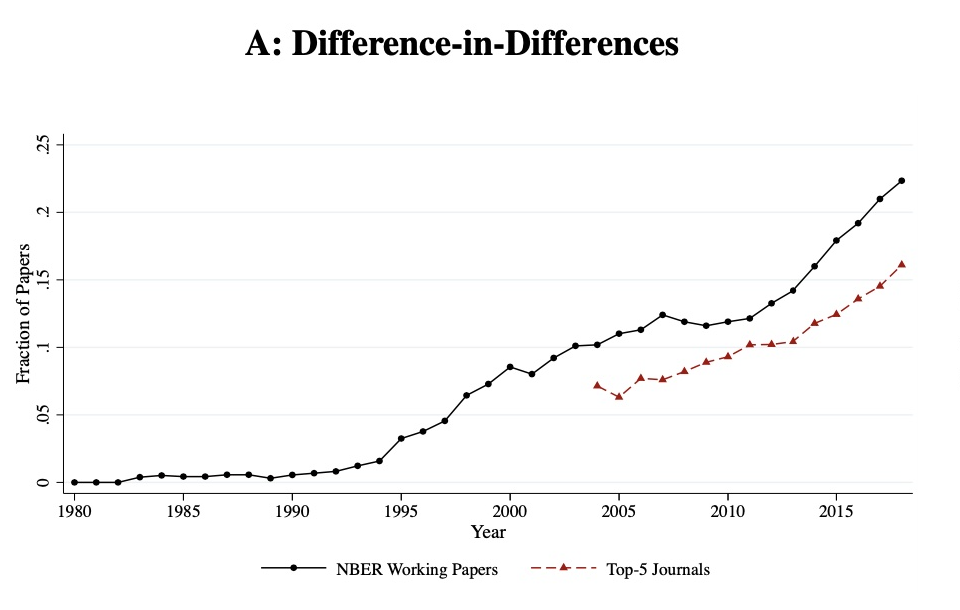
\includegraphics[scale=0.25]{./lecture_includes/currie_did.png}
	\end{figure}

\bigskip

\footnotesize


\end{frame}

\begin{frame}{Origins of diff-in-diff)}

\begin{itemize}
\item Its modern usage originates with Orley Ashenfelter and David Card in late 1970s and early 1980s work on job training programs
\item The phrase ``difference-in-differences'' is coined in a 1985 article by Ashenfelter and Card, but it was used before then
\item It seems to be the first design -- it predates the RCT by over 80 years in fact
\item It was also used in two famous public health debates in Vienna and London in the early to mid 19th century

\end{itemize}
\end{frame}




\begin{frame}{What is difference-in-differences (DiD)}

\begin{itemize}
\item DiD is when a group of units are assigned some treatment and then compared to a group of units that weren't before and after
\item One of the most widely used quasi-experimental methods in economics and increasingly in industry
\item Predates the randomized experiment by 80 years, but uses basic experimental ideas about treatment and control groups (just not randomized)
\item Uses panel or repeated cross section datasets, binary treatments usually, and often covariates 
\item Does not require a linear regression model, but for reasons we will see, linear regression accommodates it (just not all specifications equally)

\end{itemize}
\end{frame}







\begin{frame}{Ignaz Semmelweis and washing hands}

\begin{itemize}
\item Early 1820s, Vienna passed legislation requiring that if a pregnant women giving birth went to a public hospital (free care), then depending on the day of week and time of day, she would be routed to either the midwife wing or the physician wing (most likely resulting in random assignment)
\item But by the 1840s, Ignaz Semmelweis noticed that pregnant women died after delivery in the (male) wing at a rate of 13-18\%, but only 3\% in the (female) midwife wing -- cause was puerperal or “childbed” fever
\item Somehow this was also we known -- women would give birth in the street rather than go to the physician if they were unlucky enough to have their water break on the wrong day and time
\end{itemize}

\end{frame}

\begin{frame}{Ignaz Semmelweis and washing hands}

\begin{itemize}
\item Ignaz Semmelweis conjectures after a lot of observation that the cause is the teaching faculty teaching anatomy using cadavers and then delivering babies \emph{without washing hands}
\item New training happens to one but not the other and Semmelweis thinks the mortality is caused by working with cadavers
\item Convinced the hospital to have physicians wash their hands in chlorine but not the midwives, creating a type of difference-in-differences design 
\end{itemize}

\end{frame}

\begin{frame}{Semmelweis diff-in-diff evidence}

	\begin{figure}
	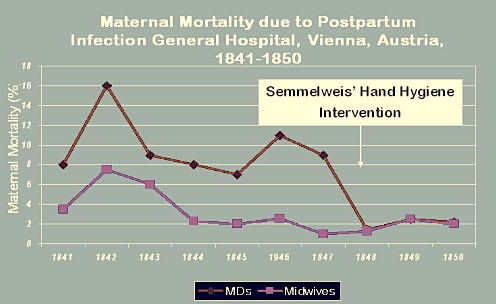
\includegraphics[scale=0.5]{./lecture_includes/semmelweis_graph.jpg}
	\end{figure}


\end{frame}

\begin{frame}{Evidence Rejected}

\begin{itemize}

\item Diff-in-diff evidence was rejected by Semmelweis' superiors claiming it was the hospital's new ventilation system
\item Dominant theory of disease spread was caused by "odors" or miasma or "humors"
\item Semmelweis began showing signs of irritability, perhaps onset of dementia, became publicly abusive, was committed to a mental hospital and within two weeks died from wounds he received while in residence
\item Despite the strength of evidence, difference-in-differences was rejected -- a theme we will see continue
\item Let's look at an illustration using a table and another story

\end{itemize}

\end{frame}






\begin{frame}{John Snow and cholera}

\begin{itemize}
\item Three major waves of cholera in the early to mid 1800s in London, largely thought to be spread by miasma (``dirty air'')
\item John Snow believed cholera was spread through the Thames water supply through an invisible creature that entered the body through food and drink, caused the body to expel water, placing the creature back in the Thames and causing epidemic waves
\item London passes ordinance requiring water utility companies to move inlet pipe further up the Thames, above the city center, but not everyone complies
\item Natural experiment: Lambeth water company moves its pipe between 1849 and 1854; Southwark and Vauxhall water company delayed
\end{itemize}

\end{frame}


\begin{frame}

	\begin{figure}
	\caption{Two water utility companies in London 1854}
	\includegraphics[scale=0.225]{./lecture_includes/lambeth.png}
	\end{figure}


\end{frame}



\begin{frame}{Difference-in-differences}

\begin{table}\centering
\scriptsize
		\caption{Lambeth and Southwark and Vauxhall, 1849 and 1854}
		\begin{center}
		\begin{tabular}{lll|lc}
		\toprule
		\multicolumn{1}{l}{\textbf{Companies}}&
		\multicolumn{1}{c}{\textbf{Time}}&
		\multicolumn{1}{c}{\textbf{Outcome}}&
		\multicolumn{1}{c}{$D_1$}&
		\multicolumn{1}{c}{$D_2$}\\
		\midrule
		Lambeth & Before & $Y=L$ \\
		& After & $Y=L + L_t + D$ & $\textcolor{red}{L_t}+D$\\
		\midrule
		& & & & $D + (\textcolor{red}{L_t}- SV_t)$ \\
		\midrule
		Southwark and Vauxhall & Before & $Y=SV$ \\
		& After & $Y=SV + SV_t$ & $SV_t$\\
		\bottomrule
		\end{tabular}
		\end{center}
	\end{table}

\begin{eqnarray*}
\widehat{\delta}_{did} = D + (\textcolor{red}{L_t}- SV_t)
\end{eqnarray*}If $\textcolor{red}{L_t}=SV_t$, then this calculation equals the effect of moving the pipe on cholera mortality.

\end{frame}







\subsection{Potential outcomes}



\begin{frame}{When is diff-in-diff causal?}

\begin{itemize}
\item Causal questions require causal notation and we will use potential outcomes
\item Potential outcomes notation is model-free explicit causal notation 
\item Rooted in the experimental design tradition and linked to statisticians Ronald Fisher, Jerzy Neyman and Don Rubin
\end{itemize}

\end{frame}




\begin{frame}{Potential outcomes notation}
	
	\begin{itemize}
	\item Let the treatment be a binary variable: $$D_{i,t} =\begin{cases} 1 \text{ if in job training program $t$} \\ 0 \text{ if not in job training program at time $t$} \end{cases}$$where $i$ indexes an individual observation, such as a person, at a particular point in time

	\end{itemize}
\end{frame}

\begin{frame}{Potential outcomes notation}
	
	\begin{itemize}

\item Potential outcomes: $$Y_{i,t}^j =\begin{cases} 1 \text{: wages at time $t$ if trained} \\ 0 \text{: wages at time $t$ if not trained} \end{cases}$$
\item Potential outcomes are \emph{a priori} real but unknown descriptions of $j$ states of the world under different treatment exposures
\item Given the treatment is binary, there are two potential outcomes for unit $i$ at time $t$: $Y^1_{i,t}$ and $Y^0_{i,t}$
\item But there are not observed until a treatment assignment is made

	\end{itemize}
\end{frame}

\begin{frame}{Realized outcomes and treatment assignment}

\begin{itemize}
\item Treatment assignment mechanisms and treatment assignment are two very different things
\item Treatment assignment is represented with the switching equation 
 $$Y_{it}=D_{it}Y_{it}^1 + (1-D_{it})Y_{it}^0$$
 \item Switching equations only show which potential outcome you're looking at, not why it and not another
 \item Switching equation is not a treatment assignment mechanism -- randomization is, rationality is, running variables are

\end{itemize}
\end{frame}





\begin{frame}{Treatment effect definitions}


	\begin{block}{Individual treatment effect}
	    The individual treatment effect,  $\delta_i$, equals $Y_i^1-Y_i^0$
	\end{block}
	
	Causal effects, or treatment effects, are simple comparisons between the two potential outcomes. 
	

	
\end{frame}

\begin{frame}{Missing Potential Outcomes}

\begin{itemize}
\item Recall the switching equation:  $$Y_{it}=D_{it}Y_{it}^1 + (1-D_{it})Y_{it}^0$$ 
\item ``Fundamental problem of causal inference'' is you need two potential outcomes but only have one
\item Some treatment assignment mechanisms let you use the untreated units as a replacement for the missing one
\end{itemize}

\end{frame}


\begin{frame}{Conditional Average Treatment Effects}	
	\begin{block}{Average Treatment Effect on the Treated (ATT)}
	The average treatment effect on the treatment group is equal to the average treatment effect conditional on being a treatment group member:
		\begin{eqnarray*}
		E[\delta|D=1]&=&E[Y^1-Y^0|D=1] \nonumber \\
		&=&E[Y^1|D=1]-\textcolor{red}{E[Y^0|D=1]}
		\end{eqnarray*}
	\end{block}
	
	\bigskip

It's the average causal effect but only for the people exposed to some intervention; notice we can't calculate it, also, because we are missing the red term

	
\end{frame}

\begin{frame}{Simple spreadsheet exercise}

Let's review basic concepts here at "WEIGHTS" tab: \url{https://docs.google.com/spreadsheets/d/10DuQqGtH_Ewea7zQoLTFYHbnvqaTVDhn2GDzq3Oa6EQ/edit?usp=sharing}

\end{frame}

\subsection{Identification, Estimation and Inference}

\begin{frame}{Orley Ashenfelter and difference-in-differences}

\begin{itemize}
\item Orley Ashenfelter ``popularized'' difference-in-differences in economics in two papers -- 1978 article and a 1985 article with David Card -- both studying job training programs
\item After graduating from Princeton, he took a job in Washington DC to work for the government
\item Got his hands on large micro data and was analyzing complex fixed effects regression models of job training program participation on wages
\item But explaining regression to normal people was difficult, so he called it ``difference-in-differences'' instead
\end{itemize}

\url{https://youtu.be/WnB3EJ8K7lg?si=BpU4Xv5p71vwHPvP&t=120}

\end{frame}


\begin{frame}{OLS Measures Four Averages and Three Subtractions}
\begin{itemize}
\item Here is the canonical DiD regression specification, sometimes called the 2x2
\end{itemize}

$$Y_{ist} = \alpha_0 + \alpha_1 Treat_{is} + \alpha_2 Post_{t} + \textcolor{blue}{\delta} (Treat_{is} \times Post_t) + \varepsilon_{ist} $$

\bigskip

\begin{itemize}
\item Orley notes that the OLS estimator of $\delta$ actually calculates ``four averages and three subtractions'' calculation are numerically identical 
\end{itemize}

\bigskip

$$\widehat{\textcolor{blue}{\delta}} = \bigg ( \overline{y}_k^{post(k)} - \overline{y}_k^{pre(k)} \bigg ) - \bigg ( \overline{y}_U^{post(k)} - \overline{y}_U^{pre(k)} \bigg ) $$

\begin{itemize}
\item Review these two calculations using \texttt{equivalence.do} in Stata to illustrate the point
\end{itemize}


\end{frame}

\begin{frame}{DiD equation is the 2x2}

Orley's ``four averages and three subtractions'' uses two groups, two time periods, or 2x2

\begin{eqnarray*}
\widehat{\delta} = \bigg ( E[Y_k|Post] - E[Y_k|Pre] \bigg ) - \bigg ( E[Y_U | Post ] - E[ Y_U | Pre] \bigg) \\
\end{eqnarray*}$k$ are the people in the job training program, $U$ are the untreated people not in the program, $Post$ is after the trainees took the class, $Pre$ is the period just before they took the class, and $E[y]$ is mean earnings. 

\bigskip

When will $\widehat{\delta}$ equal the ATT?  When will it not?

\end{frame}

\begin{frame}{Three DiD assumptions}

When it is the simple 2x2, there are three assumptions
\begin{itemize}
\item \textbf{No Anticipation}:  the ``pre'' or baseline is untreated (i.e., $Y_{t-1} = Y^0_{t-1}$ for treated units)
\item \textbf{SUTVA}: When the treatment group is treated, it does not cause the comparison group to become treated
\item \textbf{Parallel trends}:  evolution of mean $Y^0$ is the same for the treatment and comparison groups
\end{itemize}

\end{frame}



\begin{frame}{No Anticipation}

\begin{itemize}
\item  ``No anticipation''  means that the unit is not treated until it is treated
\item Rational, forward looking agents can ``turn on'' a future treatment simply by recognizing that it is coming \emph{and} changing their behavior, but not always
	\begin{itemize}
	\item \textbf{Example 1}: Tomorrow I win the lottery, but don't get paid yet. I decide to buy a new house today and a banker gives me a loan. That violates NA
	\item \textbf{Example 2}: Next year, a state lets you drive without a driver license and you know it. But you can't drive without a driver license today.  This satisfies NA.
	\end{itemize}
\item It means $Y_{i,t}=Y^0_{i,t}$ and doesn't switch to $Y^1_{i,t}$ until the treatment ``turns on'' (i.e., switching equation)

\end{itemize}


\end{frame}





\begin{frame}{SUTVA}

\begin{itemize}
\item Stable Unit Treatment Value Assumption (Imbens and Rubin 2015) focuses on what happens when in our analysis we are combining units (versus defining treatment effects)
	\begin{enumerate}
	\item \textbf{No Interference}: a treated unit cannot impact a control unit such that their potential outcomes change (unstable treatment value)
	\item \textbf{No hidden variation in treatment}: When units are indexed to receive a treatment, their dose is the same as someone else with that same index
	\item \textbf{Scale}: If scaling causes interference or changes inputs in production process, then \#1 or \#2 are violated
	\end{enumerate}
\item Shifts from defining treatment effects to estimating them, which means being careful about who is the control group, how you define treatments and what questions can and cannot be answered with this method
\end{itemize}

\end{frame}


\begin{frame}{Role of assumptions}

\begin{itemize}
\item Parallel trends is the most commonly known assumption of those three
\item But without no anticipation and SUTVA, the interpretation of difference-in-differences becomes very complex -- even with parallel trends
\item But let's start with the simple case with NA and SUTVA so that we can see parallel trends

\end{itemize}

\end{frame}



\begin{frame}{No Anticipation}

\begin{itemize}
\item Post-treatment outcome for the treated group is treated so $Y=Y^1$ in the post period for the treatment group
\end{itemize}

\begin{eqnarray*}
\widehat{\delta} = \bigg ( E[Y^1_k|Post] - \textcolor{red}{E[Y^0_k|Pre]} \bigg ) - \bigg ( E[Y_U | Post ] - E[ Y_U | Pre] \bigg) \\
\end{eqnarray*}

\begin{itemize}
\item But if the baseline is untreated, then $Y_i=Y^0_i$ at baseline
\item No Anticipation simply means that even though the treatment will occur, it has not yet occurred at baseline for all practical purposes (foreknowledge or not)
\end{itemize}


\end{frame}





\begin{frame}{SUTVA and never treated}

\begin{itemize}
\item When the treatment occurs to treated group in the post period, SUTVA means that did not cause the potential outcome to change for the comparison group
\end{itemize}

\begin{eqnarray*}
\widehat{\delta} = \bigg ( E[Y^1_k|Post] - \textcolor{black}{E[Y^0_k|Pre]} \bigg ) - \bigg ( \textcolor{red}{E[Y^0_U | Post ] - E[ Y^0_U | Pre] }\bigg) \\
\end{eqnarray*}

\begin{itemize}
\item SUTVA violations will have similar issues to when we use an already-treated group as a comparison, as we'll see
\end{itemize}


\end{frame}




\begin{frame}{Replace with potential outcomes and add a zero}

\begin{itemize}
\item Use the switching equation and replace all realized outcomes with potential outcomes assuming NA and SUTVA
\item Then add zero
\end{itemize}

\begin{eqnarray*}
\widehat{\delta} &=& \bigg ( \underbrace{E[Y^1_k|Post] - E[Y^0_k|Pre] \bigg ) - \bigg ( E[Y^0_U | Post ] - E[ Y^0_U | Pre]}_{\mathclap{\text{Switching equation}}} \bigg)  \\
&&+ \underbrace{\textcolor{red}{E[Y_k^0 |Post] - E[Y^0_k | Post]}}_{\mathclap{\text{Adding zero}}} 
\end{eqnarray*}

\end{frame}

\begin{frame}{Parallel trends bias}

\begin{itemize}
\item Rearrange the terms into the ATT plus the parallel trends bias term
\item Find the units satisfying NA and SUTVA and notice that both assumptions are nested inside the parallel trends assumption
\end{itemize}

\begin{eqnarray*}
\widehat{\delta} &=& \underbrace{E[Y^1_k | Post] - \textcolor{red}{E[Y^0_k | Post]}}_{\mathclap{\text{ATT}}} \\
&& + \bigg [  \underbrace{\textcolor{red}{E[Y^0_k | Post]} - E[Y^0_k | Pre] \bigg ] - \bigg [ E[Y^0_U | Post] - E[Y_U^0 | Pre] }_{\mathclap{\text{Non-parallel trends bias in 2x2 case}}} \bigg ]
\end{eqnarray*}

Notice that the parallel trends bias term is a difference-in-differences calculation


\end{frame}

\begin{frame}{Identification through parallel trends}
	

	\begin{block}{Parallel trends}
	Assume two groups, treated and comparison group, then we define parallel trends as:	 $$\textcolor{red}{E(}\textcolor{red}{\Delta Y^0_k)} = E(\Delta Y^0_U)$$
	\end{block}

\textbf{In words}: ``The \textcolor{red}{evolution of earnings for our trainees \emph{had they not trained}} is the same as the evolution of mean earnings for non-trainees''.  

\bigskip

It's in \textcolor{red}{red} because parallel trends is untestable and critically important to estimation of the ATT using any method, OLS or ``four averages and three subtractions''

	

	
\end{frame}


\begin{frame}{What is and is not parallel trends?}

\begin{itemize}
\item Parallel trends does \emph{not} mean treatments were randomly assigned (though random assignment guarantees parallel trends)
\item Parallel trends does \emph{not} require that the groups be similar at baseline on outcomes (though random assignment guarantees that would be)
\item Parallel trends \emph{does} require that the comparison group follows a trend in outcomes that is approximately the same as the counterfactual trend of the treatment group (what would have had happened had the treatment not occurred)
\end{itemize}

\end{frame}

\begin{frame}{No Anticipation Violation}

\begin{itemize}
\item Assume NA is violated; simply replace $Y^0_k$ at baseline with \textcolor{blue}{$Y^1_k$} instead
\end{itemize}


\begin{eqnarray*}
\widehat{\delta} &=& \bigg ( E[Y^1_k|Post] - \textcolor{blue}{E[Y^1_k|Pre]} \bigg ) - \bigg ( E[Y^0_U | Post ] - E[ Y^0_U | Pre] \bigg) \\
\end{eqnarray*}

\begin{itemize}
\item What does losing NA cost us?
\end{itemize}


\end{frame}


\begin{frame}{No Anticipation Violation}

\begin{eqnarray*}
\widehat{\delta} &=& \bigg ( \underbrace{E[Y^1_k|Post] - \textcolor{blue}{E[Y^1_k|Pre] }\bigg ) - \bigg ( E[Y^0_U | Post ] - E[ Y^0_U | Pre]}_{\mathclap{\text{Switching equation}}} \bigg)  \\
&&+ \underbrace{\textcolor{red}{E[Y_k^0 |Post] - E[Y^0_k | Post]}}_{\mathclap{\text{Adding zero}}} 
\end{eqnarray*}


\end{frame}

\begin{frame}{No Anticipation Violation}

\begin{eqnarray*}
\widehat{\delta} &=& \underbrace{E[Y^1_k | Post] - \textcolor{red}{E[Y^0_k | Post]}}_{\mathclap{\text{ATT}}} \\
&& + \bigg [  \underbrace{\textcolor{red}{E[Y^0_k | Post]} - \textcolor{blue}{E[Y^1_k | Pre]} \bigg ] - \bigg [ \textcolor{black}{E[Y^0_U | Post]} - E[Y_U^0 | Pre] }_{\mathclap{\text{This is not the parallel trends term}}} \bigg ]
\end{eqnarray*}

``Parallel trends'' refers to  $\Delta E[Y^0_k]$ and $\Delta E[Y^0_U]$.  But that's not what is in that line.  So let's add another zero to try and get a standard parallel trends term

\end{frame}

\begin{frame}{No Anticipation Violation}

\begin{eqnarray*}
\widehat{\delta} &=& \underbrace{E[Y^1_k | Post] - \textcolor{red}{E[Y^0_k | Post]}}_{\mathclap{\text{ATT}}} \\
&& + \bigg [  \underbrace{\textcolor{red}{E[Y^0_k | Post]} - \textcolor{blue}{E[Y^1_k | Pre]} \bigg ] - \bigg [ \textcolor{black}{E[Y^0_U | Post]} - E[Y_U^0 | Pre] }_{\mathclap{\text{This is not the parallel trends term}}} \bigg ] \\
&& + \underbrace{ \textcolor{red}{E[Y^0_k|Pre] - E[Y^0_k|Pre]}}_{\mathclap{\text{Add another zero}}}
\end{eqnarray*} Now rearrange the second and third row

\end{frame}

\begin{frame}{No Anticipation Violation}

\begin{eqnarray*}
\widehat{\delta} &=& \underbrace{E[Y^1_k | Post] - \textcolor{red}{E[Y^0_k | Post]}}_{\mathclap{\text{ATT}}} \\
&& + \bigg [  \underbrace{\textcolor{red}{E[Y^0_k | Post]} - \textcolor{red}{E[Y^0_k | Pre]} \bigg ] - \bigg [ \textcolor{black}{E[Y^0_U | Post]} - E[Y_U^0 | Pre] }_{\mathclap{\text{Parallel trends term}}} \bigg ] \\
&& + \underbrace{ \textcolor{red}{E[Y^0_k|Pre]} - \textcolor{blue}{E[Y^1_k|Pre]}}_{\mathclap{\text{Reversed treatment effect?}}}
\end{eqnarray*}. Now let's switch the order of the third row

\end{frame}

\begin{frame}{No Anticipation Violation}

\begin{eqnarray*}
\widehat{\delta} &=& \underbrace{E[Y^1_k | Post] - \textcolor{red}{E[Y^0_k | Post]}}_{\mathclap{\text{Post treatment ATT}}} \\
&& + \bigg [  \underbrace{\textcolor{red}{E[Y^0_k | Post]} - \textcolor{red}{E[Y^0_k | Pre]} \bigg ] - \bigg [ \textcolor{black}{E[Y^0_U | Post]} - E[Y_U^0 | Pre] }_{\mathclap{\text{Parallel trends term}}} \bigg ] \\
&& - \bigg [ \underbrace{ \textcolor{blue}{E[Y^1_k|Pre]} - \textcolor{red}{E[Y^0_k|Pre]}}_{\mathclap{\text{Baseline ATT}}} \bigg ]
\end{eqnarray*}. 

\end{frame}





\begin{frame}{No Anticipation Violation}

If the baseline period is treated, then the simple 2x2 identifies the following three terms:

\begin{eqnarray*}
\delta &=& ATT_k(Post) + \text{Non PT bias}  - ATT_k(Pre)
\end{eqnarray*}

If you use a treated unit at baseline, then DiD will be attenuated towards zero, and if treatment effects are constant, DiD will equal zero

\bigskip 

Let's look in \texttt{na.do}.

\end{frame}




\begin{frame}{Using already treated comparison group}


\begin{eqnarray*}
\widehat{\delta} &=& \bigg ( E[Y_k|Post] - E[Y_k|Pre] \bigg ) - \bigg ( E[Y_U | Post ] - E[ Y_U | Pre] \bigg) \\
\end{eqnarray*}What if the $U$ group had always been treated in both periods? Is parallel trends enough to identify the ATT?

\bigskip

Replace realized outcomes with potential outcomes and rewrite using the ``add zero'' trick we did.  We will review the answer tomorrow morning.

\bigskip

Hint: You know you're not done until you see a standard parallel trends assumption


\end{frame}











\begin{frame}{Understanding parallel trends through worksheets}

Before we move into regression, let's go through a simple exercise to really pin down these core ideas with simple calculations

\bigskip 

\url{https://docs.google.com/spreadsheets/d/1onabpc14JdrGo6NFv0zCWo-nuWDLLV2L1qNogDT9SBw/edit?usp=sharing}

\end{frame}



\begin{frame}{Summarizing}

\begin{itemize}

\item Lots of restrictions placed on difference-in-differences
	\begin{itemize}
	\item NA: you chose a baseline that is not treated
	\item SUTVA: your comparison group is never treated during the course of the calculations
	\item PT: your comparison group has a trend in $E[Y^0]$ that is the same as the counterfactual 
	\end{itemize}
\item Only when you have NA and SUTVA does DiD equal ATT + PT
\item But it's crucial to remember: DiD and ATT are not the same thing

\end{itemize}

\end{frame}








\begin{frame}{OLS Specification}
	
	\begin{itemize}
	\item Simple DiD equation will identify ATT under parallel trends
	\item But so will a particular OLS specification (two groups and no covariates)
	\item OLS was historically preferred because
		\begin{itemize}
		\item OLS estimates the ATT under parallel trends
		\item Easy to calculate the standard errors
		\item Easy to include multiple periods
		\end{itemize}
	\item People liked it also because of differential timing, continuous treatments and covariates, but those are more complex so we address them later
	\end{itemize}
\end{frame}

\begin{frame}{Minimum wages}

\begin{itemize}
\item Card and Krueger (1994) have a famous study estimating causal effect of minimum wages on employment
\item  New Jersey raises its minimum wage in April 1992 (between February and November) but neighboring Pennsylvania does not
\item Using DiD, they do not find a negative effect of the minimum wage on employment leading to complex reactions from economists
\item Orley's describes his understanding of people's reaction to the paper.  \\ \url{https://youtu.be/MOtbuRX4eyQ?t=1882}
\end{itemize}

\end{frame}

\begin{frame}
	\begin{figure}
	
\includegraphics[scale=0.5]{./lecture_includes/minwage_whore}
	\end{figure}
\end{frame}


\begin{frame}{Reaction to the paper}


Lots of anecdotes in this interview with Card, but here are just two.  First, Card and Krueger received a lot of personal hostility from their peers (1:07 to 1:10)

\bigskip

\url{https://youtu.be/1soLdywFb_Q?si=laAVYf_E2KBZKywG&t=4020}

\bigskip

Later Card says Sherwin Rosen accused them of having an agenda.  But the worst is what happens to Alan Krueger maybe (1:16 to 1:17)

\bigskip

\url{https://youtu.be/1soLdywFb_Q?si=jsb8h50ZosGDnKrv&t=4556}




\end{frame}

\begin{frame}{Card on that study}

\begin{quote}
``I’ve subsequently stayed away from the minimum wage literature for a number of reasons. First, it cost me a lot of friends. People that I had known for many years, for instance, some of the ones I met at my first job at the University of Chicago, became very angry or disappointed. They thought that in publishing our work we were being traitors to the cause of economics as a whole.''
\end{quote}


\end{frame}



\begin{frame}{OLS specification of the DiD equation}
	
	\begin{itemize}
	\item The correctly specified OLS regression is an interaction with time and group fixed effects:$$Y_{its} = \alpha + \gamma NJ_s + \lambda d_t + \delta (NJ \times d)_{st} + \varepsilon_{its}$$
		\begin{itemize}
		\item NJ is a dummy equal to 1 if the observation is from NJ
		\item d is a dummy equal to 1 if the observation is from November (the post period)
		\end{itemize}
	\item This equation takes the following values
		\begin{itemize}
		\item PA Pre: $\alpha$
		\item PA Post: $\alpha + \lambda$
		\item NJ Pre: $\alpha + \gamma$
		\item NJ Post: $\alpha + \gamma + \lambda + \delta$
		\end{itemize}
	\item DiD equation: (NJ Post - NJ Pre) - (PA Post - PA Pre) $= \delta$
	\end{itemize}
\end{frame}




\begin{frame}[plain]
	$$Y_{ist} = \alpha + \gamma NJ_s + \lambda d_t + \delta(NJ\times d)_{st} + \varepsilon_{ist}$$
	\begin{figure}
	\includegraphics[scale=0.90]{./lecture_includes/waldinger_dd_5.pdf}
	\end{figure}
\end{frame}


\begin{frame}[plain]
	$$Y_{ist} = \alpha + \gamma NJ_s + \lambda d_t + \delta(NJ\times d)_{st} + \varepsilon_{ist}$$
	\begin{figure}
	\includegraphics[scale=0.90]{./lecture_includes/waldinger_dd_5.pdf}
	\end{figure}

Notice how OLS is ``imputing'' $E[Y^0|D=1,Post]$ for the treatment group in the post period? It is only ``correct'', though, if parallel trends is a good approximation

\end{frame}




\begin{frame}{Inference in DID}
	\begin{itemize}
	\item When dealing with clustered data, a crucial issue is the calculating the standard errors associated with the sampling variance of your estimator
 	\item Correlated errors occur when the unobserved errors are correlated within a cluster.
	\item Failing to account for correlated errors can lead to misleading inference, biased standard errors and higher over rejection
	\end{itemize}
\end{frame}


\begin{frame}{Serial correlation creates problems}
  \begin{itemize}
	\item  Bertrand, Duflo and Mullainathan (2004) show that conventional standard errors will often severely understate the standard deviation of the estimators
	\item They proposed three solutions: bootstrapping, allowing for arbitrary clustered correlations, and a third approach that is very strange
	    \item Clustering is typically recommended at the aggregate level where the entire treatment occurred at the aggregate level 
	    \item It is considered a more conservative approach to inference

  \end{itemize}
\end{frame}








%\begin{frame}{Computing Cluster-Robust Standard Errors}
%  \begin{enumerate}
%    \item Run your regression to get \( u \) and \( \hat{Y} \).
%    \item Calculate cluster-level residuals \( \hat{u}_c \).
%    \item Calculate the "meat" (as in bread-meat-bread sandwich) \( M \) as \( \sum_c X_c^\prime \hat{u}_c \hat{u}_c^\prime X_c \).
%    \item Your standard error covariance matrix is \( \hat{V} = (X^\prime X)^{-1} M (X^\prime X)^{-1} \).
%  \end{enumerate}
  
%  \bigskip
  
%  Mixtape reference (chapter 2): \url{https://mixtape.scunning.com/02-probability\_and\_regression\#cluster-robust-standard-errors}
%\end{frame}

%\begin{frame}{Compressing Into a Single Number}
%  \begin{itemize}
%    \item Diagonal elements of \( \hat{V} \) contain variances for each coefficient.
%    \item Standard errors are the square root of these diagonal elements.
%    \item Non-diagonal elements are used for hypothesis tests and confidence intervals for combinations of coefficients.
%  \end{itemize}
%\end{frame}


\begin{frame}{Summarizing}

\begin{itemize}
\item Diff-in-diff isn't necessarily causal: it requires SUTVA, NA, parallel trends and an untreated comparison group
\item But if you have all of those, then difference-in-differences identifies the ATT
\item We will assume for now you have SUTVA, NA and an untreated comparison group as they are the ones easier to rationalize
\item But parallel trends is untestable since we never observe \textcolor{red}{$E[Y^0_k|Post]$} so how do approach this?
\item We'll discuss some general practical advice and propose some solutions
\end{itemize}

\end{frame}



\section{Parallel Trends Violations}

\subsection{Main Results, Proof and Evidence}


\begin{frame}{Main Results Depend on Untestable Assumption}

	\begin{itemize}
	\item You put your regression results in a table and call it your main results and you claim they're causal under parallel trends (which is true)
	\item But what can you do to provide evidence that parallel trends is believable?
	\item Unfortunately, parallel trends is not testable because you are missing \textcolor{red}{$E[Y^0_k|Post]$} 
	\item There's a few standard things that are always done, plus some new things, and we will discuss them all
	\end{itemize}

\end{frame}


\begin{frame}{Evidence for Parallel Trends}

	\begin{itemize}

	\item Think a prosecutor arguing against a defense attorney to convince a judge and jury
	\item The claim the defendant is guilty but the claim is not the evidence -- it's more like an assertion
	\item The evidence is the smoking gun, the fingerprints, the eye witnesses, the footprints in the mud outside the house
	\item If your claim is supported by weak evidence, then no one \emph{should} convict -- it would be borderline corruption if they did 
	\item Our evidence will be bite, falsifications, mechanisms and event study data visualization 
	\end{itemize}

\end{frame}








\subsection{Parallel Trends and Event Studies}



\begin{frame}{Event studies have become mandatory in DiD}

	\begin{figure}
	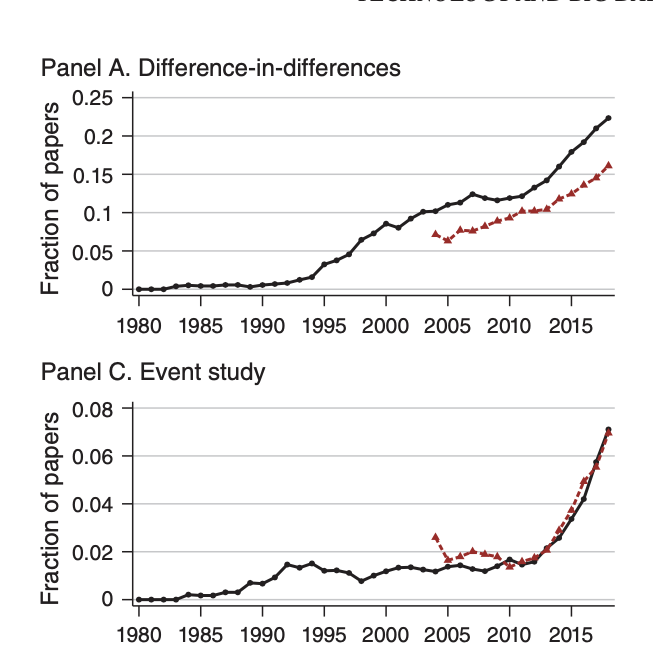
\includegraphics[scale=0.5]{./lecture_includes/currie_eventstudy.png}
	\end{figure}

\end{frame}




\begin{frame}{Creating event studies}

\begin{itemize}

\item Event studies mean different things to different people -- in finance and accounting, they are methods for evaluating abnormal stock market returns and historically were fairly parametric
\item At some point in the early 2000s, economists start plotting the treatment and control outcomes both before and after the point of treatment
\item Reasoning is ``maybe if the two groups had comparable trends before treatment, they would have after the treatment had the treatment not happened''
\item People have done it different ways, but regardless of the way, the reason is the same

\end{itemize}

\end{frame}



\begin{frame}{Plot the raw data when there's only two groups}

	\begin{figure}
	\includegraphics[scale=2.5]{./lecture_includes/waldinger_dd_6.pdf}
	\end{figure}

\end{frame}


\begin{frame}{Event study regression}
	
	\begin{itemize}
	\item Alternatively, present estimated coefficients from a dynamic regression specification:
 $$Y_{it} = \alpha + \sum_{\tau=-2}^{-q}\mu_{\tau} (D_i \times \tau_t) + \sum_{\tau=0}^m\delta_{\tau} (D_i \times \tau_t) + \tau_t + D_i + \varepsilon_{it}$$
		\begin{itemize}
		\item With a simple 2x2, event study regressions simply interact the treatment dummy ($D_i$) with calendar year dummies ($\tau_t$)
		\item There are $q$ pre-treatment leads and $m$ post treatment lags 
		\item Each coefficient is a separate ``four averages and three subtractions'' for that period relative to the dropped baseline
		\end{itemize}
\item  Typically you'll plot the coefficients and 95\% CI on all leads and lags, usually with a vertical line marking just before treatment happened
	\end{itemize}
\end{frame}

\begin{frame}{Pre-treatment DiD coefficient}

\begin{eqnarray*}
\widehat{\mu}_{t-2} &=& \bigg [  \underbrace{\textcolor{black}{E[Y^0_k | t-2]} - E[Y^0_k | t-1] \bigg ] - \bigg [ E[Y^0_U | t-2] - E[Y_U^0 | t-1] }_{\mathclap{\text{Differential trends in pre-treatment $\Delta E[Y^0]$}}} \bigg ]
\end{eqnarray*}

\bigskip

\begin{itemize}
\item  Under NA, all pre-treatment periods are untreated, therefore by definition $Y=Y^0$ for all pre-treatment periods
\item If NA then ATT$=$0 in all pre-periods, therefore the pre-treatment coefficients \emph{only} equal the differential trend
\item Unlike parallel trends (which uses post-treatment missing potential outcomes), this is testable
\item And if the pre-treatment coefficients are zero, interpreting the post-treatment coefficients as ATT becomes more plausible

\end{itemize}

\end{frame}


\begin{frame}{Two types of evidence for parallel trends}

\begin{enumerate}
\item \textbf{Event study}: Only examines whether the two groups were comparable on trends pre-treatment
\item \textbf{Falsification}: Only examines whether a similar group who was not eligible for the treatment shows similar patterns as found with the treatment group (more on this later)
\end{enumerate}

\bigskip

Let's look at an example involving a diff-in-diff application involving near elderly mortality in the United States and health insurance, but we will just focus on the event studies

\end{frame}


\begin{frame}{Example US Healthcare}

\begin{itemize}
\item United States does not have universal healthcare except for the elderly and the very poor
\item Elderly get Medicare and must be 65 or older; the very poor get Medicaid so long as their income is below some threshold
\item Barack Obama signature policy achievement was at the Affordable Care Act which gave incentives to states to raise that threshold
\item Some states did; some did not
\end{itemize}

\end{frame}



\begin{frame}{Medicaid and Affordable Care Act example}

\begin{figure}
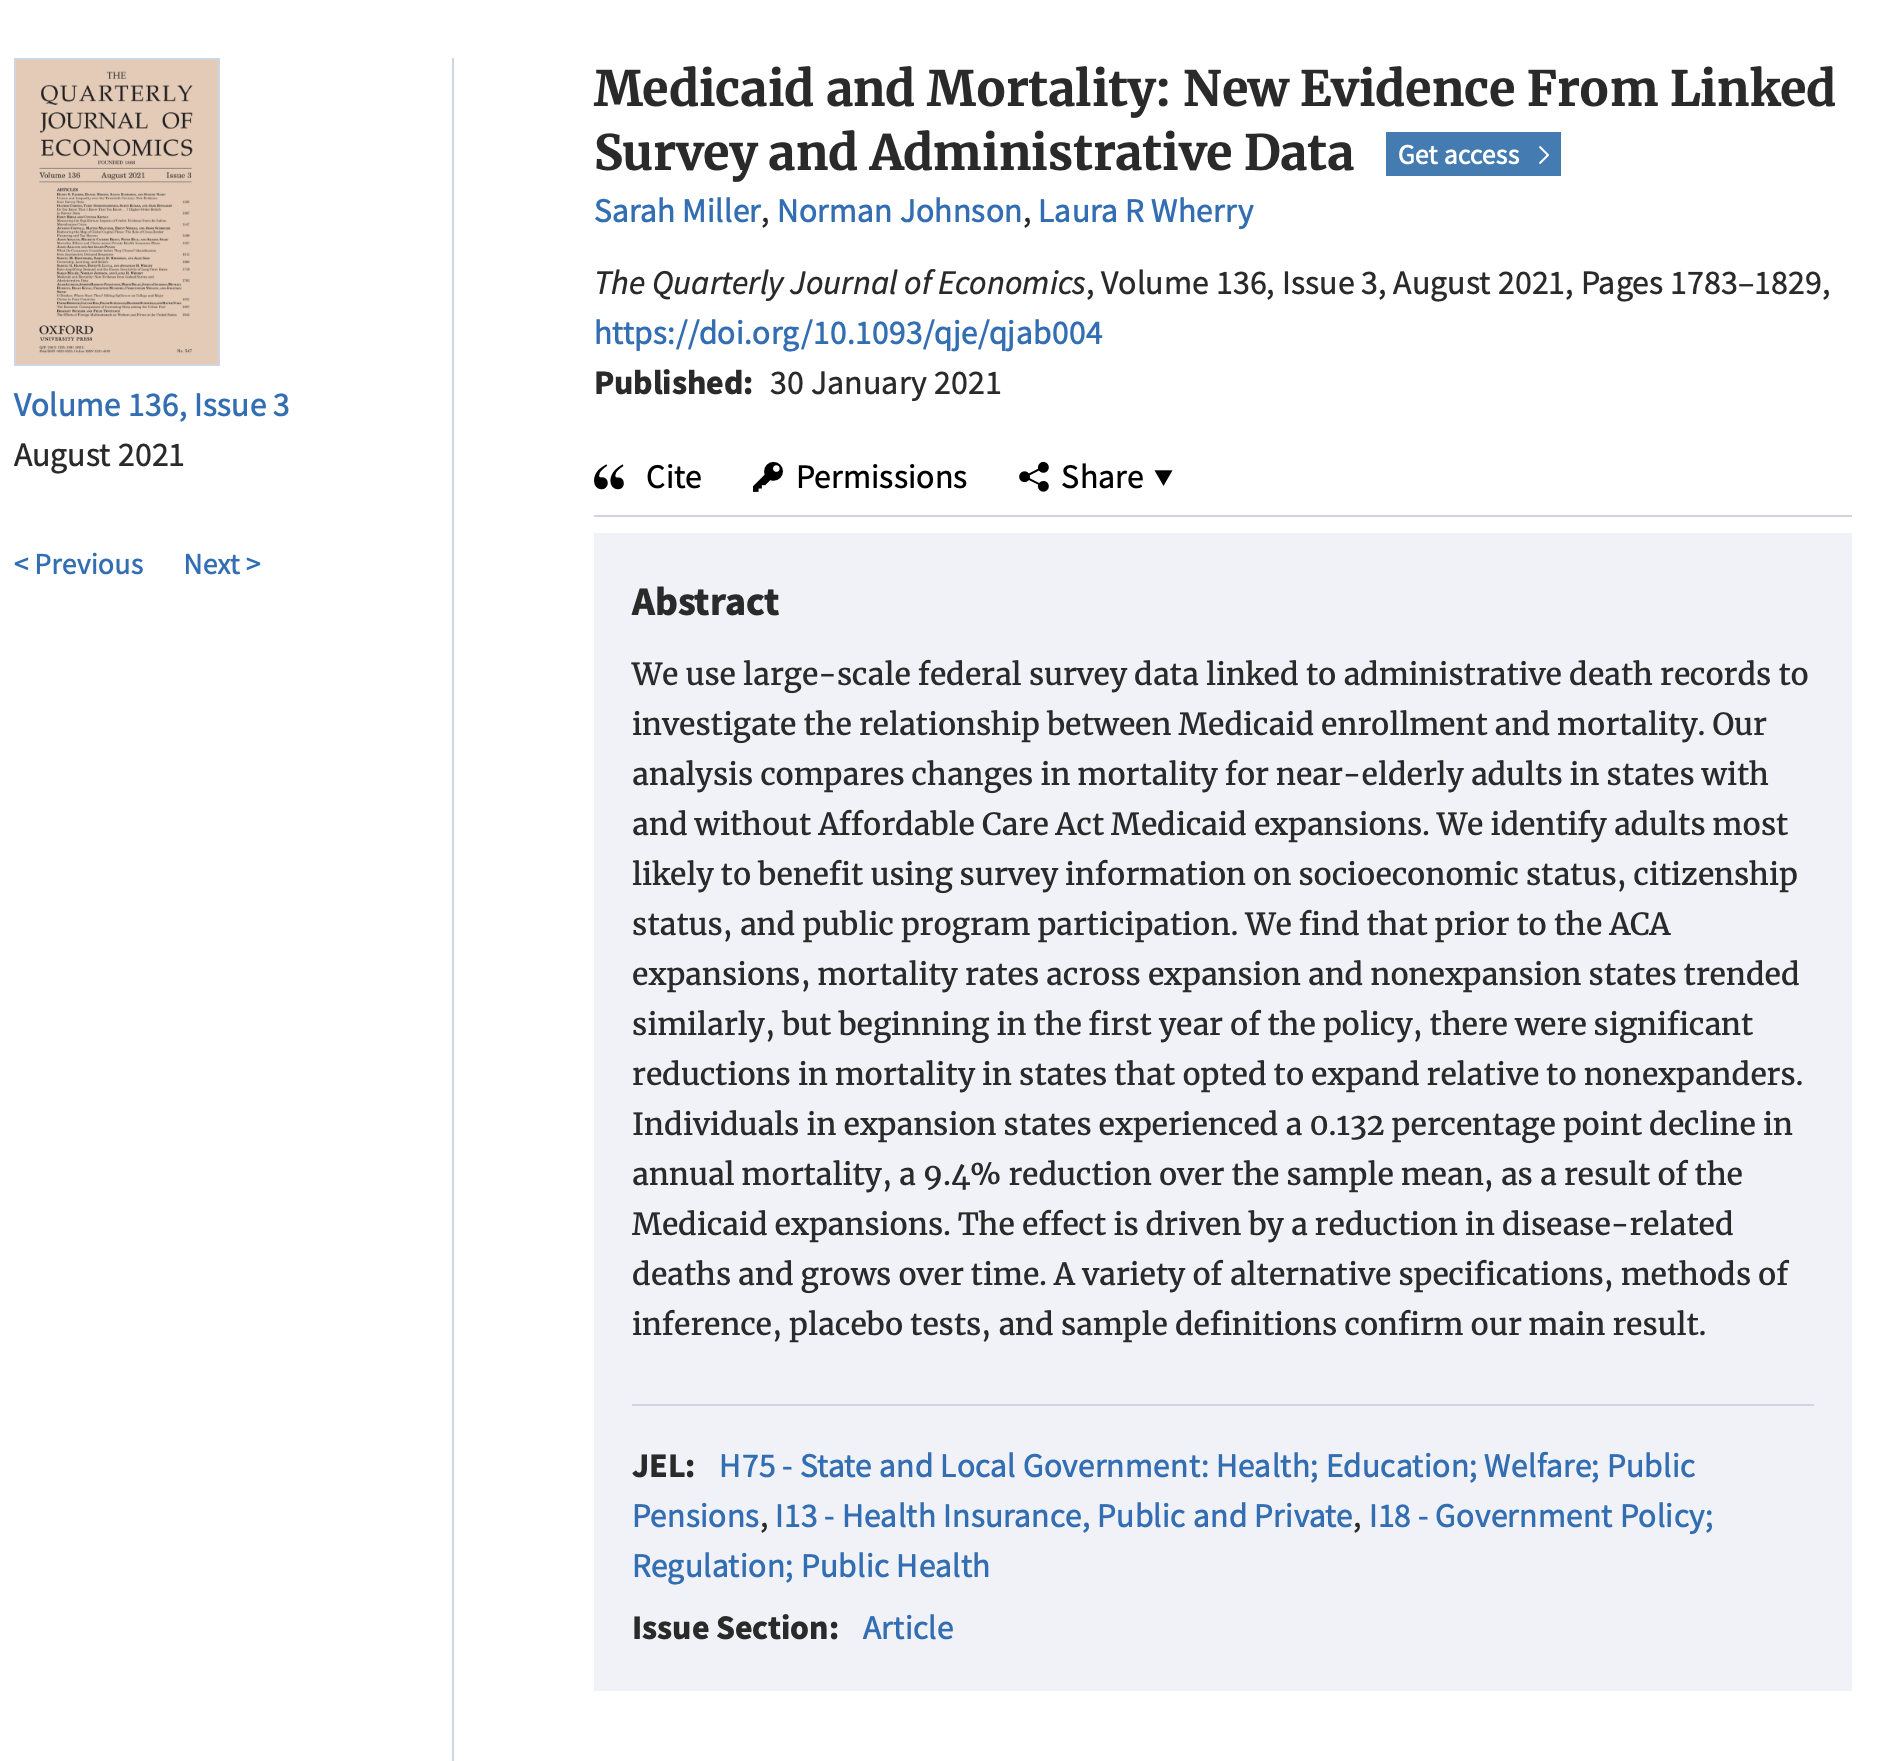
\includegraphics[scale=0.25]{./lecture_includes/medicaid_qje}
\end{figure}

\end{frame}


\begin{frame}{Their Evidence versus Their Result}

Miller, Johnson and Wherry used difference-in-differences to evaluate its effect on mortality on the ``near elderly'' (younger than 65) and provide strong evidence supporting the credibility of their main results

\begin{enumerate}
\item \textbf{Bite} -- they will show that the expansion shifted people into Medicaid and out of uninsured status
\item \textcolor{black}{\textbf{Placebos}} -- they show that there's no effect of Medicaid on a similar group that didn't enroll
\item \textbf{Event study} -- they will lean hard on those dynamic plots
\item \textcolor{red}{\textbf{Main results}} -- with all of this, they will show Medicaid expansion caused near elderly mortality to fall
\item \textcolor{black}{\textbf{Mechanisms}} -- they think they can show it's coming from people treating diseases causing mortality declines to compound over time
\end{enumerate}

\end{frame}

\begin{frame}{Bite}

\begin{itemize}
\item Bite in this context means when US states made Medicaid more generous, people got on Medicaid who would not have been on it otherwise
\item And as a bonus, would not have been insured at all without it
\item Bite does not provide evidence for parallel trends, but provides credibility overall because if there is no evidence people enrolled in a program, then how can the program have any effect on them?
\item Their bite evidence is presented entirely with event studies
\end{itemize}

\end{frame}


\begin{frame}{Bite evidence \#1 }

	\begin{figure}
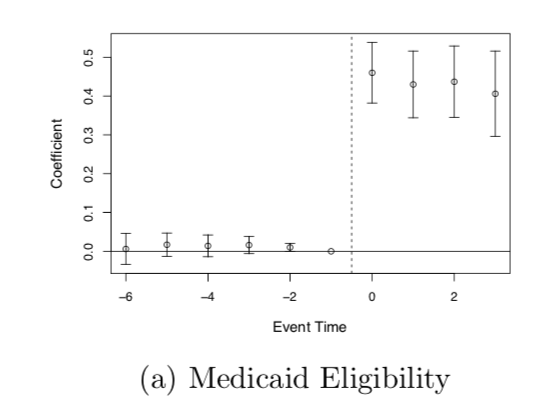
\includegraphics[scale=0.5]{./lecture_includes/Miller_Medicaid1.png}
	\end{figure}

\end{frame}

\begin{frame}{Bite evidence \#2 }

	\begin{figure}
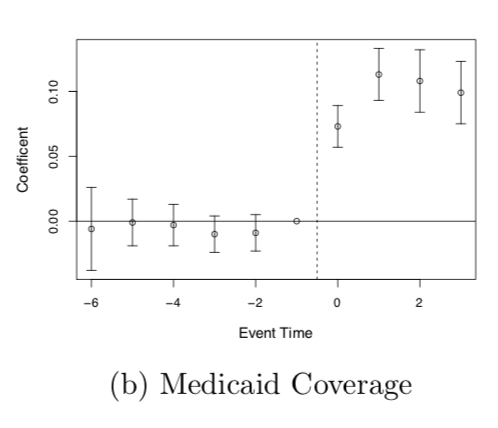
\includegraphics[scale=0.5]{./lecture_includes/Miller_Medicaid2.png}
	\end{figure}

\end{frame}


\begin{frame}{Bite evidence \#3 }

	\begin{figure}
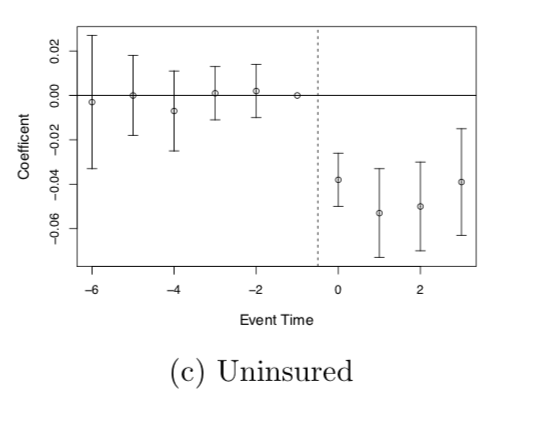
\includegraphics[scale=0.5]{./lecture_includes/Miller_Medicaid3.png}
	\end{figure}

\end{frame}

\begin{frame}{Summarizing bite}

\begin{itemize}

\item Seems clear that when states made healthcare insurance more generous, more people enrolled (around 5-6pp more)
\item Some probably switched from private insurance to public insurance
\item But not all -- the last figure showed a 4-6pp reduction in uninsured status
\item Pre-trends look great, too -- the treatment and comparison states appear to have been following \emph{identical} trends, probably because this subpopulation of poor people are not changing or changing behavior a lot anywhere

\end{itemize}

\end{frame}





\begin{frame}{Falsification}

\begin{itemize}

\item Event studies tell us something about whether two groups were on similar trends before the treatment, but they don't say what would have happened after
\item Miller, Johnson and Wherry use a falsification in addition to event studies to see if unobserved confounders might be happening in the post-treatment period in the expanding states
\item They'll look at 65 and older coverage and mortality
\item They're already on Medicare so they shouldn't get on Medicaid, and they're very similar to the ``near elderly'' so they should have similar confounders
\end{itemize}

\end{frame}

\begin{frame}{Falsifications on 65 year old and older}

	\begin{figure}
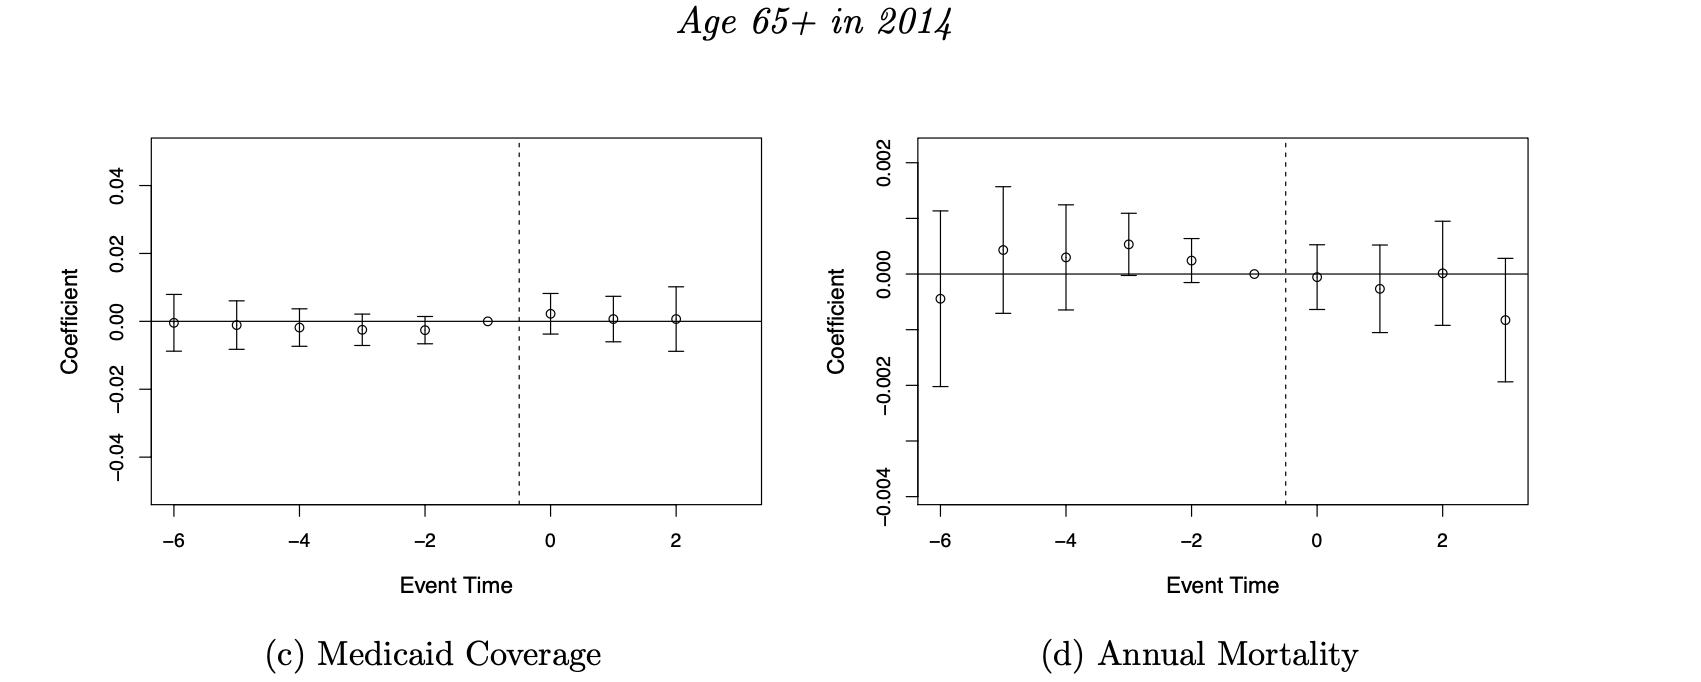
\includegraphics[scale=0.425]{./lecture_includes/placebo_medicaid}
	\end{figure}

\end{frame}

\begin{frame}{Main result}

\begin{itemize}

\item Finally they focus on the main result -- and there's more in the paper than I'm showing
\item Event study plots with same specification as the rest allowing us to look at the pre-trends and the post-treatment coefficients
\item If parallel trends holds, then the post-treatment coefficients are interpreted as ATT parameter estimates for each time period
\item The result alone isn't nearly as strong the result in combination with the rest, but it could still be wrong as parallel trends is ultimately not verfiable
\end{itemize}

\end{frame}



\begin{frame}{Near elderly mortality and Medicaid expansion}

	\begin{figure}
	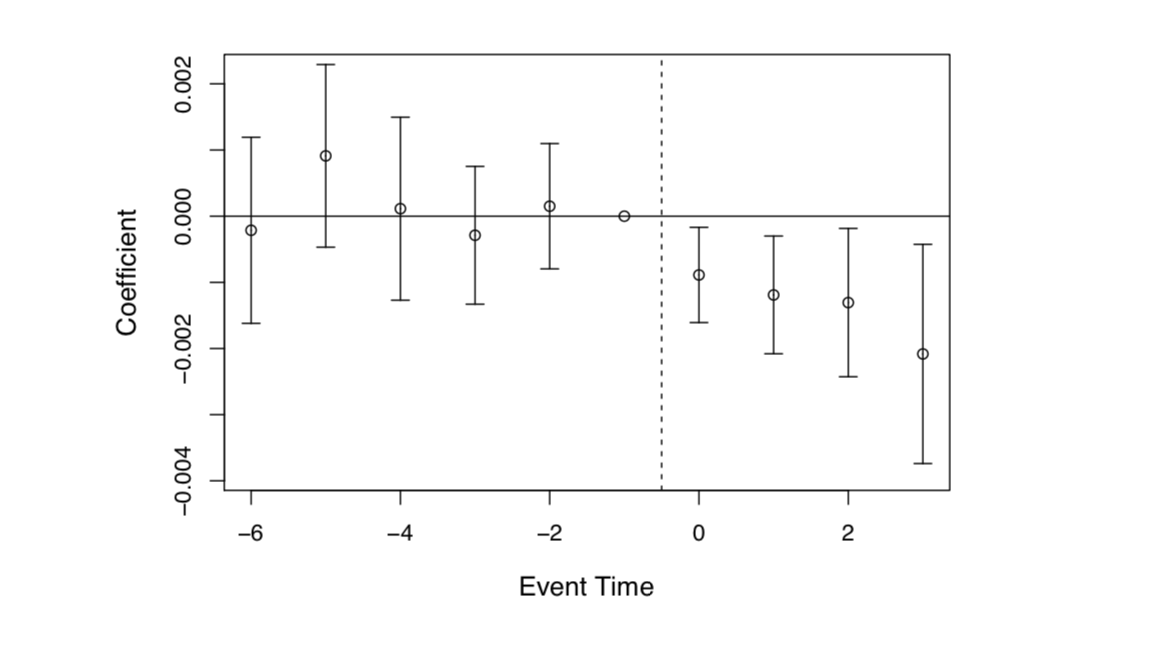
\includegraphics[scale=0.3]{./lecture_includes/Miller_Medicaid4.png}
	\end{figure}

\end{frame}

\begin{frame}{Main results and mechanism}

\begin{itemize}
\item \textcolor{black}{Main results}: They translate that percentage point reduction into a 9.2\% reduction in mean mortality among the near-elderly
\item \textcolor{black}{Mechanism}: They attribute this effect to a reduction in disease-related deaths that grew over time 
\item Notice how they did so much with simple data visualization (event studies); let's just look at how those are created now
\end{itemize}

\end{frame}

\begin{frame}{Making event study}

\begin{itemize}
\item Recall the specification when there is only one treatment group and one comparison group

 $$Y_{it} = \alpha + \sum_{\tau=-2}^{-q}\mu_{\tau} (D_i \times \tau_t) + \sum_{\tau=0}^m\delta_{\tau} (D_i \times \tau_t) + \tau_t + D_i + \varepsilon_{it}$$

\item Regression fully interacts treatment group indicator with calendar time indicators
\item Be sure to use an untreated group-period as the baseline (e.g., $t-1$) otherwise NA is violated and DID will be attenuated (minus baseline ATT)
\item There is some Stata and R code ( \texttt{simple\_eventstudy.do} ) at the repo to illustrate how to create this using a dataset on homicides and a treatment indicator
\end{itemize}

\end{frame}


\begin{frame}{Manually creating the event study}

	\begin{figure}
	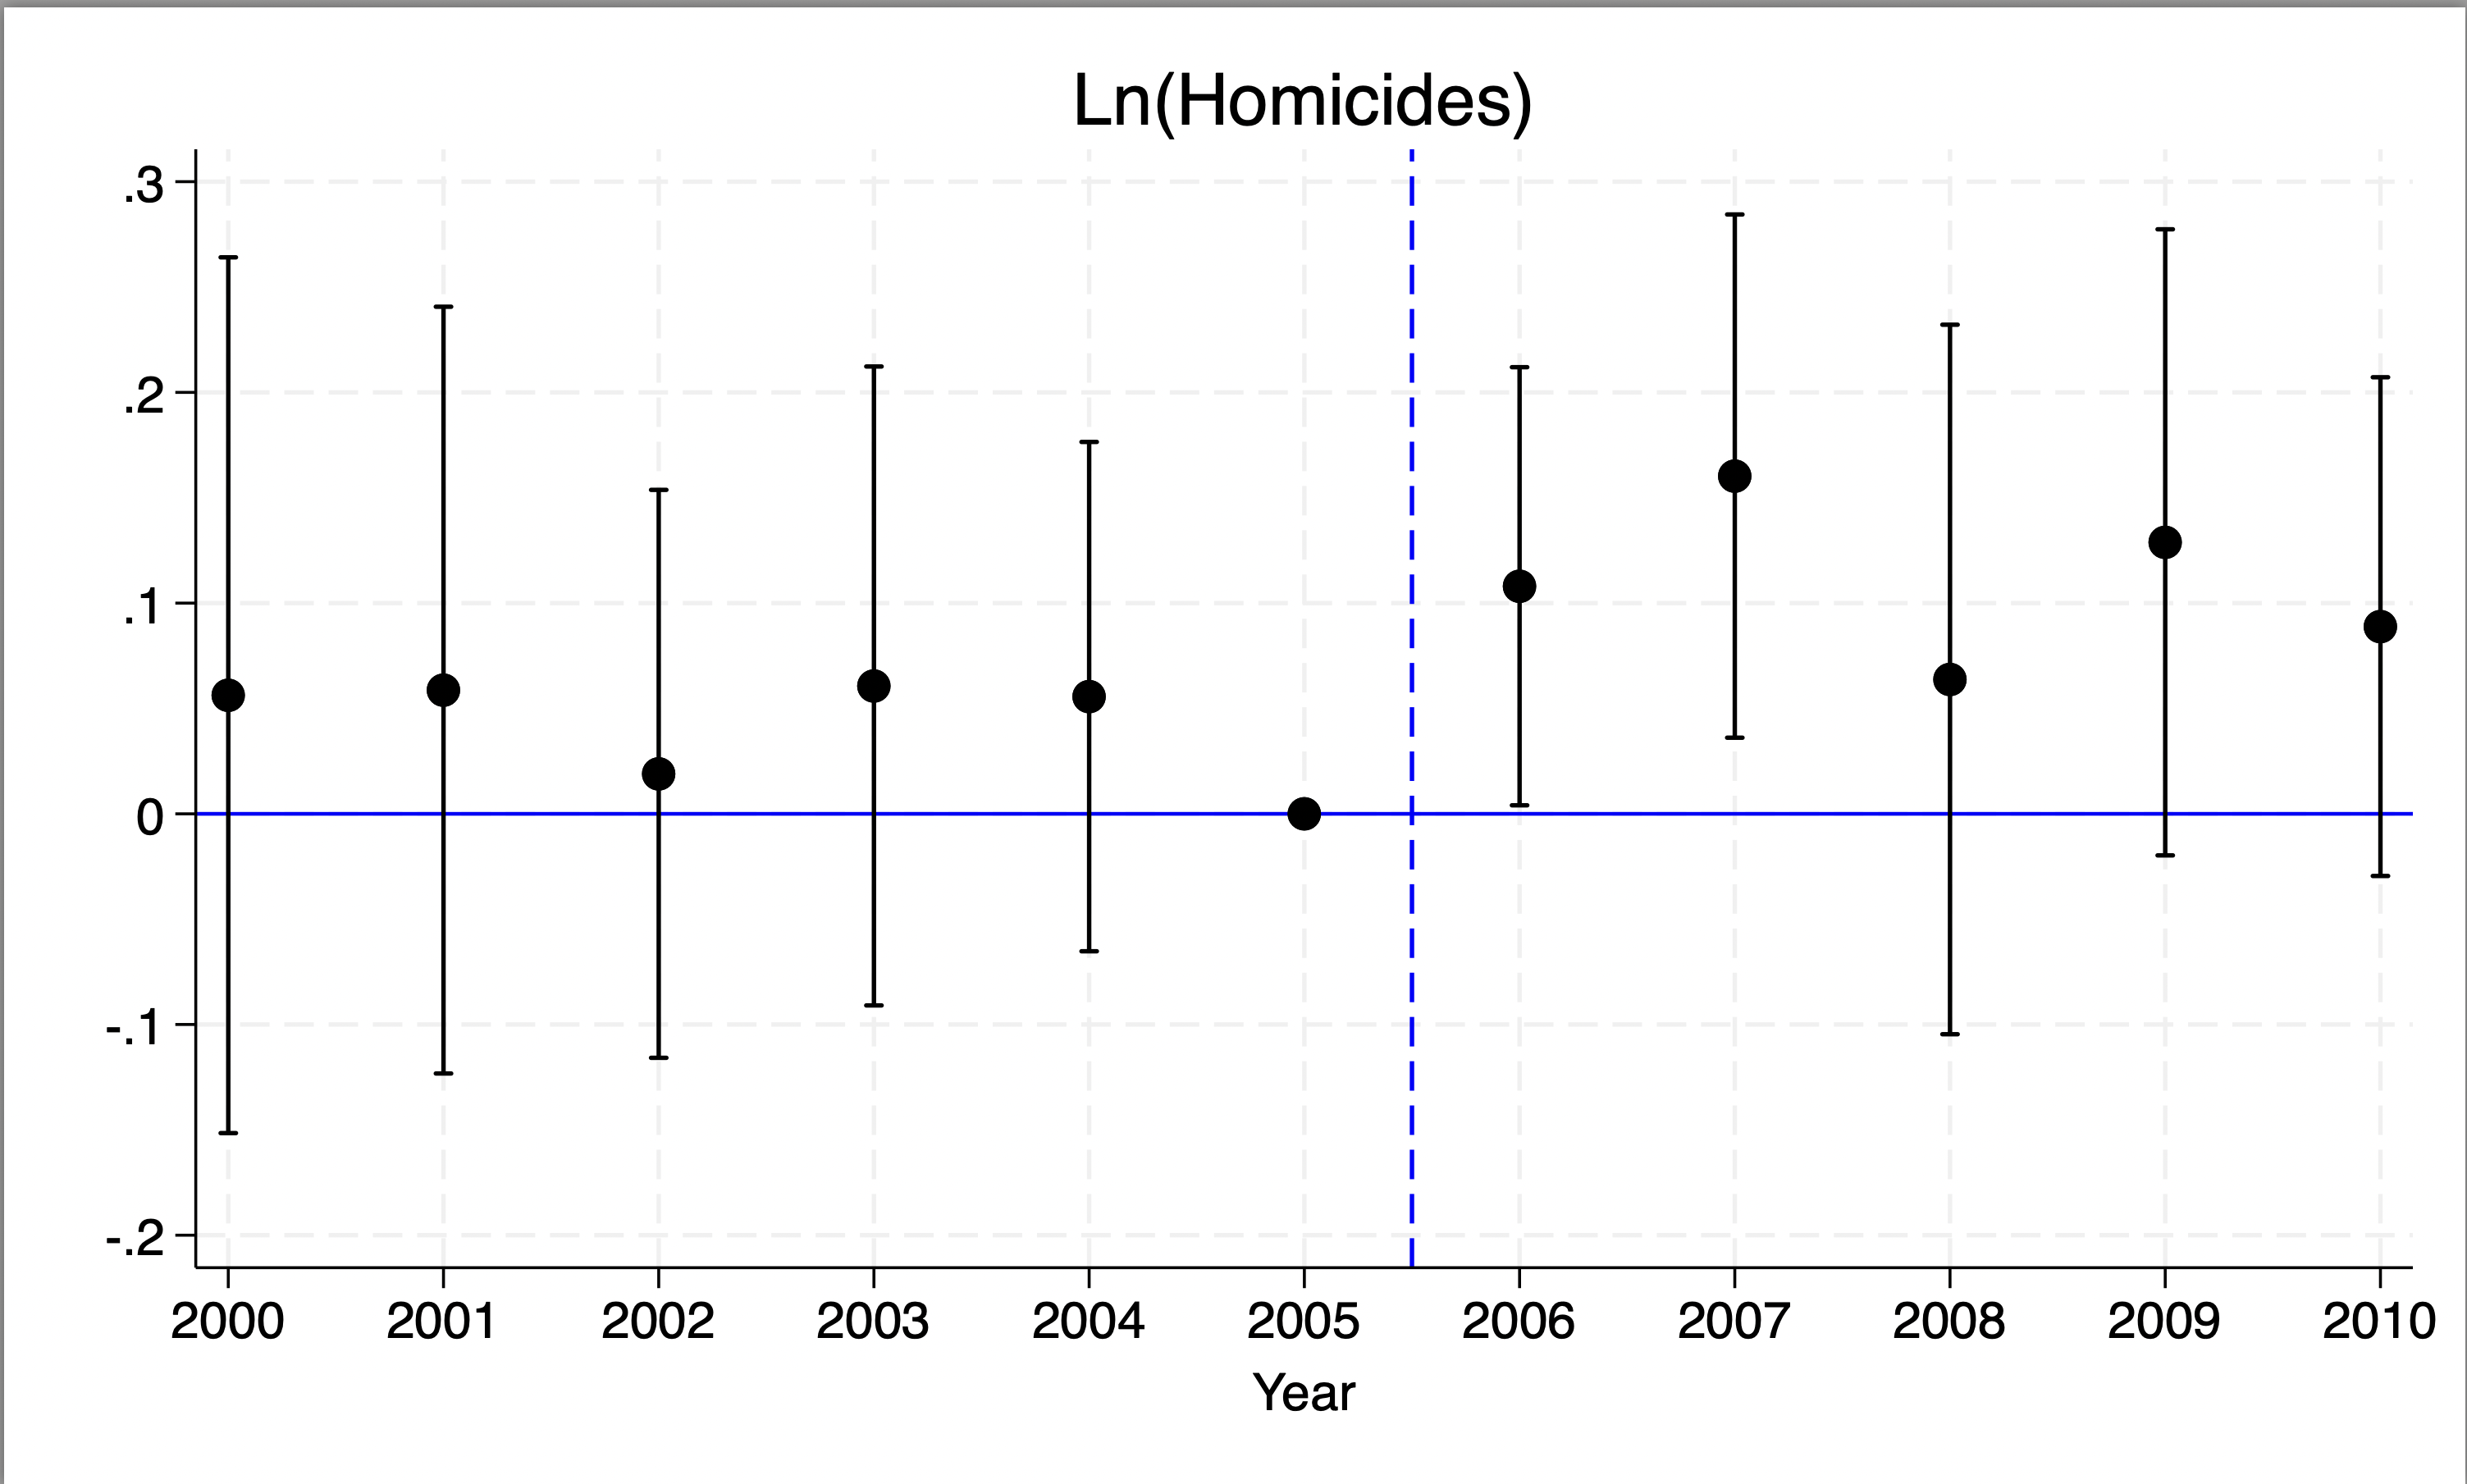
\includegraphics[scale=0.20]{./lecture_includes/simple_eventstudy_manual}
	\end{figure}

\end{frame}




\begin{frame}{Creating the event study with Ben Jann's \texttt{coefplot}}

	\begin{figure}
	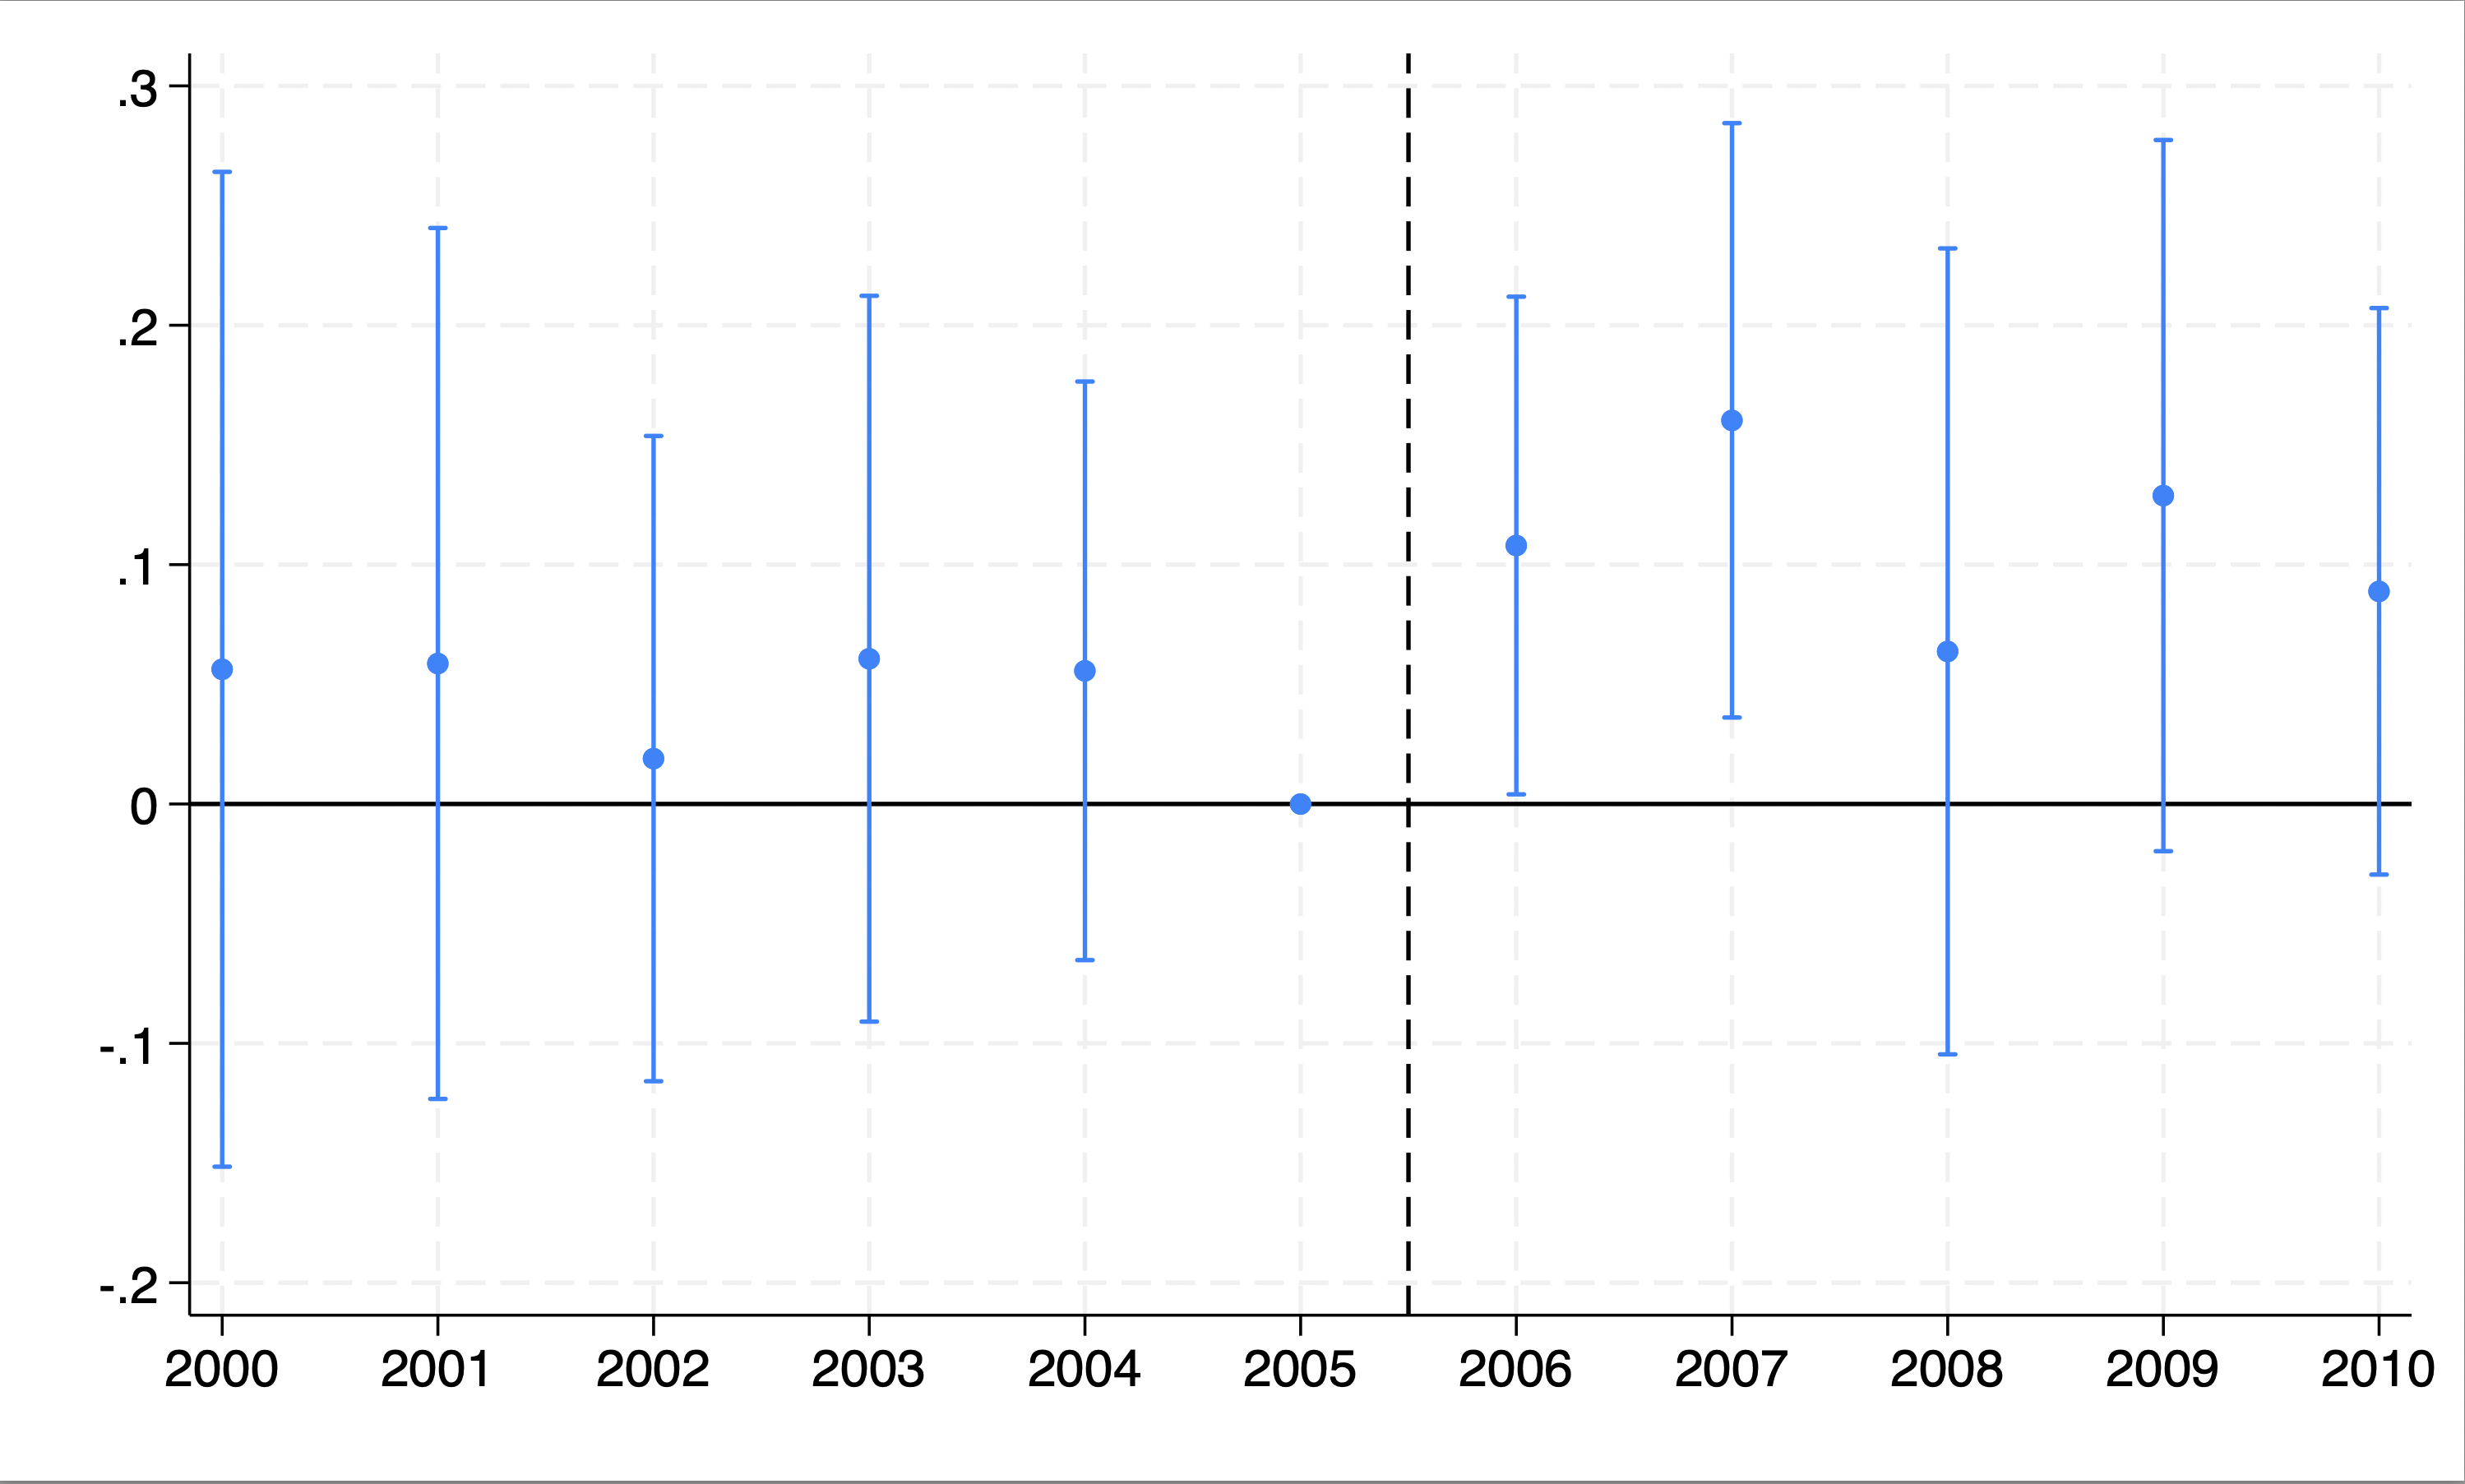
\includegraphics[scale=0.20]{./lecture_includes/simple_eventstudy.png}
	\end{figure}

\end{frame}






\subsection{Problems with Pre-trends: Low Power and Bounding}


\begin{frame}{Biased diff-in-diff}

\begin{itemize}

\item But what if your pre-trends look horrible?  What can you do?
\item There are two options I'll discuss now: one uses bounding (Rambachan and Roth 2024) and the other uses triple differences
\item Tomorrow we will discuss using covariates to address a biased diff-in-diff

\end{itemize}

\end{frame}

\begin{frame}{Low Power}

\begin{itemize}

\item Parallel trends plus NA and SUTVA is sufficient to identify the ATT using diff-in-diff
\item And testing for whether differential trends between the two groups existed in the pre-period is a common sense way of assessing the plausibility of the parallel trends assumption
\item But has limitations: one of them has to do with power and one has to do with a kind of selection bias created by only analyzing cases without statistically significant pre-trends
\item This is from Jon Roth's work, which I will briefly summarize

\end{itemize}

\end{frame}

\begin{frame}{Low Power}

\begin{itemize}

\item Even if the pre-trends were not zero, you may not have the power needed to detect it statistically
\item Jon in his 2022 AER: Insights, ``Pre-test with Caution: Event-study Estimates After Testing for Parallel Trends'' discusses this in detail
\item Let me illustrate with one of my recent papers the problem to consider: Cunningham, DeAngelo and Tripp (2024), ``Did Craigslist's Erotic Services Reduce Female Homicide and Rape?'', \emph{Journal of Human Resources}
\item Study uses the staggered rollout of Craigslist's ``erotic services'' section of its website, used for matching sex workers and clients, to identify its effect on female victimization with twoway fixed effects and matrix completion


\end{itemize}

\end{frame}


\begin{frame}{Event study from my research}
    \begin{figure}
        \centering
        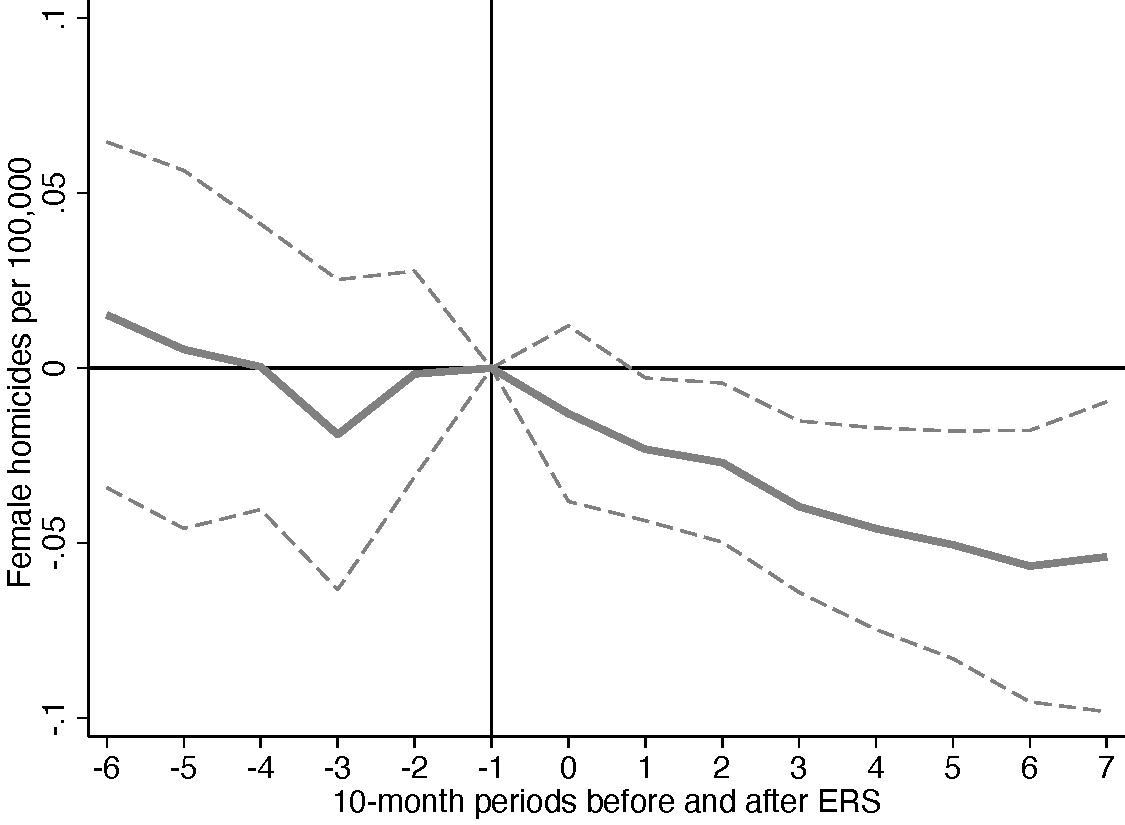
\includegraphics[width=0.6\textwidth, height=0.6\textheight, keepaspectratio]{./lecture_includes/es_homicides_twfe.pdf}
    \end{figure}
    \begin{itemize}
        \item We weren't able to reject the null that there were no pre-trends (p-value of 0.5).
    \end{itemize}
\end{frame}

\begin{frame}{Event study from my research}
    \begin{figure}
        \centering
        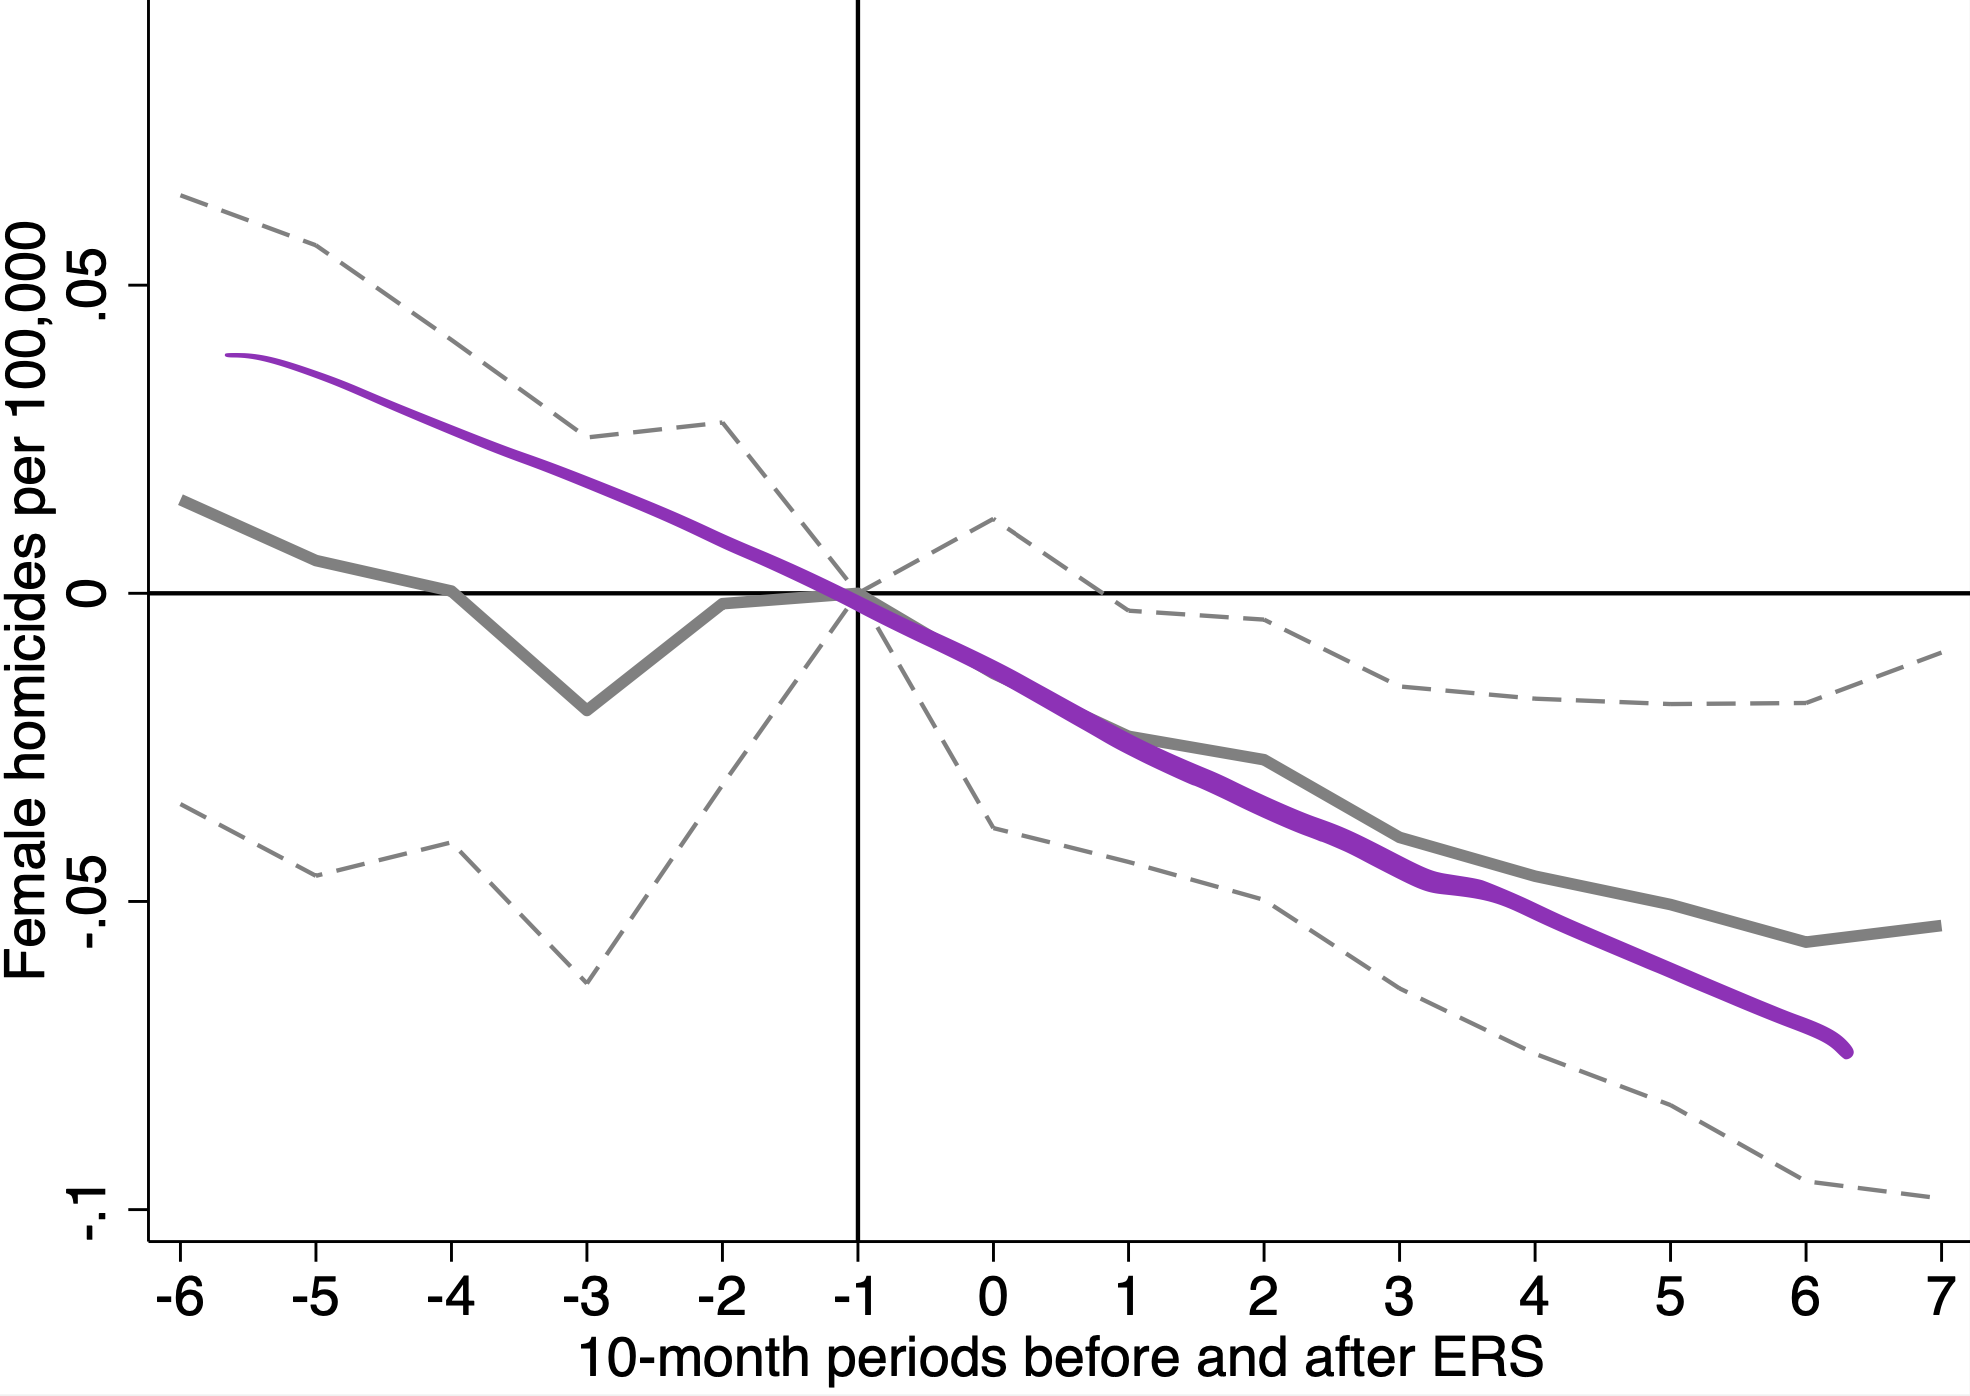
\includegraphics[width=0.6\textwidth, height=0.6\textheight, keepaspectratio]{./lecture_includes/es_lowpower.png}
    \end{figure}
    \begin{itemize}
        \item However, we couldn't have rejected the null of a linear trend either due to large CI.
	\item So even if pre-trends were non-zero, we may fail to detect it statistically
    \end{itemize}
\end{frame}

\begin{frame}{Simulations}

\begin{itemize}
\item Roth (2022) had simulations calibrated to papers published in the AER, AEJ: Applied and AEJ: Policy between 2014 and 2018
\item 70 papers contained and event study plot; he focused on 12 with available data
\item He evaluated properties of standard estimates/CIs under linear violations of parallel trends against which conventional tests have limited power and found:
	\begin{enumerate}
	\item Bias was often of the same magnitude as the estimated treatment effect
	\item CIs substantially undercovered in many cases
	\end{enumerate}
\item There are limitations to pre-trends testing due to low power -- you may not find significant pre-trends even if parallel trends itself is being violated
\end{itemize}

\end{frame}

\begin{frame}{Summary of Pretrends Package}
    \begin{itemize}
        \item The \texttt{pretrends} package offers tools for power calculations for pre-trends tests and visualization of potential parallel trends violations, based on Roth (2022, AER:Insights) (\url{https://github.com/jonathandroth/pretrends})
        \item It helps assess the power of pre-trends tests by calculating the ex ante power to detect violations and visualizing these on an event-study plot.
        \item For a more comprehensive solution to parallel trends violations, consider using the HonestDiD package, which forms confidence intervals for treatment effects accounting for pre-treatment violations.
    \end{itemize}
\end{frame}

\begin{frame}{Quote from Rambachan and Roth (2024, REstud)}
    \begin{figure}
        \centering
        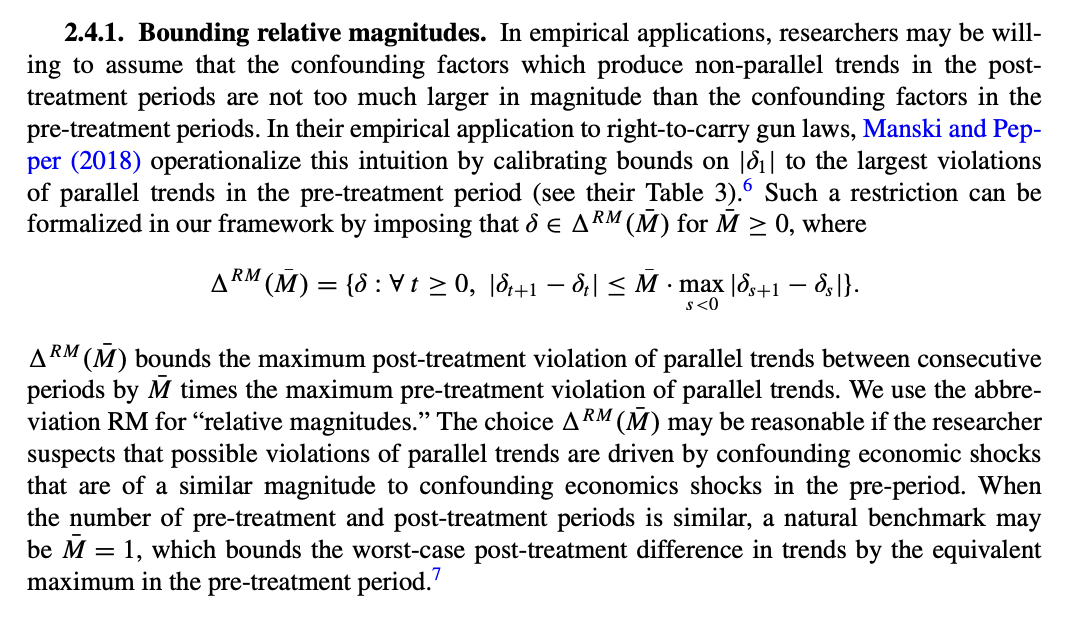
\includegraphics[width=0.8\textwidth, height=0.8\textheight, keepaspectratio]{./lecture_includes/rr_quote}
    \end{figure}
\end{frame}


\begin{frame}{Bounds on Relative Magnitudes}

\begin{itemize}

\item Rambachan and Roth (2024), ``A More Credible Approach to Parallel Trends'', \emph{Review of Economic Studies}
\item Intuition, recall, in pre-trends testing is that the pre-trends are informative about counterfactual post-treatment trends
\item How different would the counterfactual trend have to be from the pre-trends to erase your conclusion about the treatment effects?
\item They use this restriction to bound the treatment effect under these imposed restrictions

\end{itemize}

\end{frame}

\begin{frame}{Medicaid's Effect on Insurance Coverage}
    \begin{figure}
        \centering
        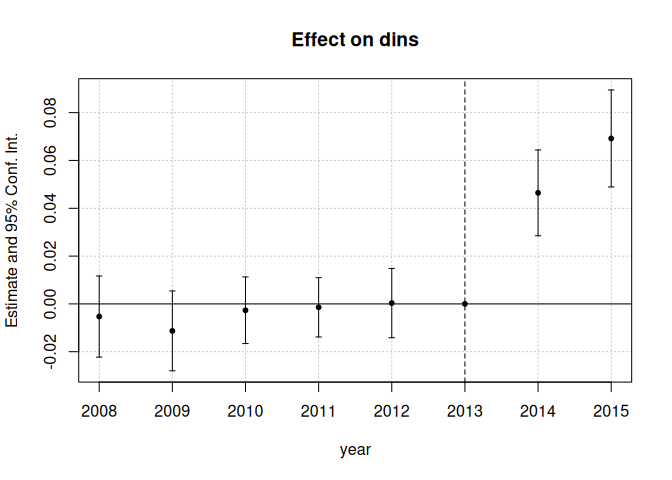
\includegraphics[width=0.6\textwidth, height=0.6\textheight, keepaspectratio]{./lecture_includes/original_miller.png}
    \end{figure}
    \begin{itemize}
        \item Note the negative effect in 2009 of around -1pp
    \end{itemize}
\end{frame}


\begin{frame}{Event study from my research}
    \begin{figure}
        \centering
        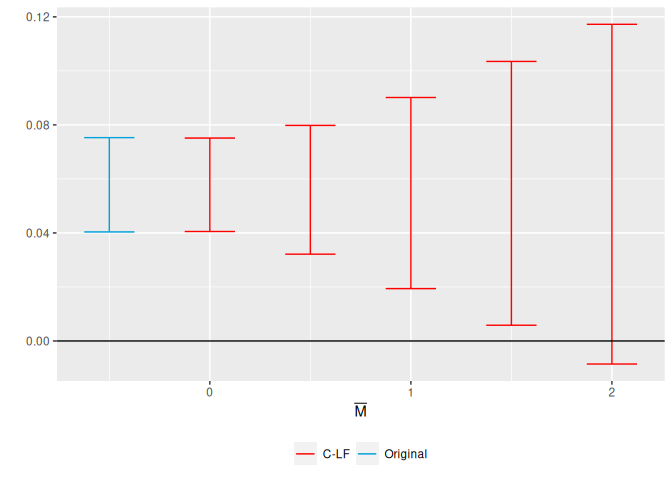
\includegraphics[width=0.6\textwidth, height=0.6\textheight, keepaspectratio]{./lecture_includes/bounding_miller.png}
    \end{figure}
    \begin{itemize}
	\item Impose that the post-treatment violation of parallel trends is no more than some constant $\overline{M}$ which you can set to 0 (original) or some factor (e.g., 2 or no more than twice as large)
	\item We can rule out a null effect unless we allow for violations of PT of 2x larger than the max in the pre-period
    \end{itemize}
\end{frame}






\subsection{Triple differences}


\begin{frame}{Triple differences}

\begin{itemize}
\item Another core methodology is the triple differences design (Gruber 1994)
\item Many people equate triple differences with falsification exercise, but actually it isn't that -- it is it's own design
\item You use triple differences when diff-if-diff is biased and parallel trends is violated
\item Is is \emph{not} falsification; rather it is a research design with assumptions which are new
\end{itemize}

\end{frame}






\begin{frame}{Biased diff-in-diff \#1}

\begin{table}\centering
\scriptsize
		\caption{Biased diff-in-diff \#1: comparing states}
		\begin{center}
		\begin{tabular}{lll|lc}
		\toprule
		\multicolumn{1}{l}{\textbf{States}}&
		\multicolumn{1}{c}{\textbf{Period}}&
		\multicolumn{1}{c}{\textbf{Outcomes}}&
		\multicolumn{1}{c}{$D_1$}&
		\multicolumn{1}{c}{$D_2$}\\
		\midrule
		Experimental states & Before & $Y=NJ$ \\
		& After & $Y=NJ + NJ_t + D$ & $\textcolor{red}{NJ_t}+D$\\
		\midrule
		& & & & $D + (\textcolor{red}{NJ_t}- PA_t)$ \\
		\midrule
		Non-experimental  & Before & $Y=PA$ \\
		states& After & $Y=PA + PA_t$ & $PA_t$\\
		\bottomrule
		\end{tabular}
		\end{center}
	\end{table}

\begin{eqnarray*}
\widehat{\delta}^{true}_{did} = D + (\textcolor{red}{NJ_t}- PA_t)
\end{eqnarray*}The ATT is D. Assume, though, that parallel trends does not hold, $(\textcolor{red}{NJ_t} \neq PA_t)$

\end{frame}


\begin{frame}{Biased Placebo diff-in-diff}

\begin{table}\centering
\scriptsize
		\caption{Biased placebo diff-in-diff: comparing states but single men and older women}
		\begin{center}
		\begin{tabular}{lll|lc}
		\toprule
		\multicolumn{1}{l}{\textbf{States}}&
		\multicolumn{1}{c}{\textbf{Period}}&
		\multicolumn{1}{c}{\textbf{Outcomes}}&
		\multicolumn{1}{c}{$D_1$}&
		\multicolumn{1}{c}{$D_2$}\\
		\midrule
		Experimental states & Before & $Y=NJ$ \\
		& After & $Y=NJ + NJ_t $ & $\textcolor{red}{NJ_t}$\\
		\midrule
		& & & & $ (\textcolor{red}{NJ_t}- PA_t)$ \\
		\midrule
		Non-experimental  & Before & $Y=PA$ \\
		states& After & $Y=PA + PA_t$ & $PA_t$\\
		\bottomrule
		\end{tabular}
		\end{center}
	\end{table}

\begin{eqnarray*}
\widehat{\delta}^{placebo}_{did} = (\textcolor{red}{NJ_t}- PA_t)
\end{eqnarray*}Assume that parallel trends does not hold, $(\textcolor{red}{NJ_t} \neq PA_t)$

\end{frame}


\begin{frame}{Two biased diff-in-diffs}

\begin{itemize}


\item Parallel trends does not hold, $(\textcolor{red}{NJ_t} \neq PA_t)$, but what if that's the same bias in our placebo DiD?
\item Then we can subtract the second from the first: $$ \widehat{\delta}_{ddd} = \widehat{\delta}^{true}_{did} - \widehat{\delta}^{placebo}_{did}$$
\item Triple differences is a ``real design'' with one parallel trends assumption: $$(\textcolor{red}{NJ_t}^{true}- PA_t^{true}) = (\textcolor{red}{NJ_t}^{placebo}- PA_t^{placebo})$$

\end{itemize}

\end{frame}

\begin{frame}{Triple differences by Gruber (1995)}
	
	\begin{figure}
	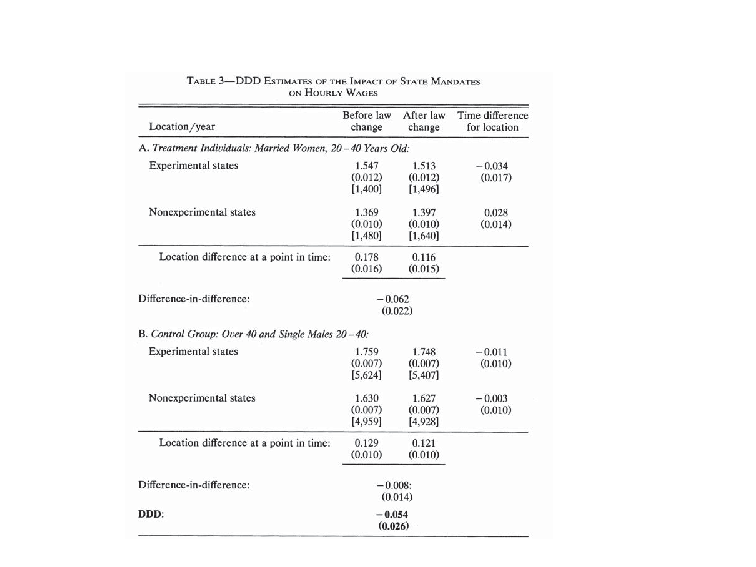
\includegraphics{./lecture_includes/gruber_ddd_3.pdf}
	\end{figure}
	
\end{frame}

\begin{frame}{Triple differences commentary}

\begin{itemize}
\item Some people think that it requires that the placebo DiD be zero, but that's incorrect

\item In Gruber's 1995 article, it isn't clear why he needed triple differences in the first place -- his triple differences yielded -0.054 which is almost the same as what he found with his first diff-in-diff (-0.062)
\item The main value of triple differences is that you use it when you believe the parallel trends assumption doesn't hold

\end{itemize}

\end{frame}


\begin{frame}[shrink=20]

\begin{table}\centering
		\caption{Difference-in-Difference-in-Differences (Gruber version)}
		\tiny
		\begin{center}
		\begin{tabular}{lll|l|lll}
		\toprule
		\multicolumn{1}{l}{\textbf{Groups}}&
		\multicolumn{1}{c}{\textbf{States}}&
		\multicolumn{1}{c}{\textbf{Period}}&
		\multicolumn{1}{c}{\textbf{Outcomes}}&
		\multicolumn{1}{c}{$D_1$}&
		\multicolumn{1}{c}{$D_2$}&
		\multicolumn{1}{c}{$D_3$}\\
		\midrule
		&&After	&$NJ+MW+\textcolor{blue}{NJ_t}+\textcolor{red}{MW_t}+D$					\\
	&Experimental			&&&$\textcolor{blue}{NJ_t}+MW_t + D$			\\
		&states&Before	&$NJ+MW$					\\
Married women 					&&&&&$D+\textcolor{blue}{NJ_t} -PA_t 	$	\\
20-40							&&&&&$$\\
    		&&After	&$PA+MW+PA_t+MW_t$					\\
	&Non-experimental		&&	&$PA_t+MW_t$				\\
		&states&Before	&$PA+MW$					\\
								\\
&&&&&&$\textcolor{black}{D}$
\\
		&&After	&$NJ+SO+NJ_t+SO_t$				\\
	&Experimental 			&&&$NJ_t+SO_t$ \\				
		&states&Before	&$NJ+SO$					\\
Single men 					&&&&&$NJ_t  - PA_t$		\\
Older women					&&&&&$$		\\
	     	&&After	&$PA+SO+PA_t+SO_t$					\\
	&Non-experimental		&&&	$PA_t+SO_t$				\\
		&states&Before	&$PA+SO$					\\
		\bottomrule
		\end{tabular}
		\end{center}
	\end{table}

\begin{center}
\textbf{Triple diff assumption}
\end{center}

$\widehat{\delta}_{DDD}= D + \underbrace{[(\textcolor{blue}{NJ^{MW}_t} - PA^{MW}_t) -( NJ^{SO}_t - PA^{SO}_t )]}_{\mathclap{\text{Equally biased  DiD \#1 and \# 2}}}$

\bigskip
Triple differences requires two diff-in-diff, from different groups, with the same bias. Parallel bias


\end{frame}







\begin{frame}{DDD in Regression}
	
	\begin{eqnarray*}
	Y_{ijt} &=&\alpha +  \beta_2 \tau_t + \beta_3 \delta_j  + \beta_4 D_i + \beta_5(\delta \times \tau)_{jt} \\
	&& +\ \beta_6(\tau \times D)_{ti} +  \beta_7(\delta \times D)_{ij} +  \textcolor{red}{\beta_8(\delta \times \tau \times  D)_{ijt}}+  \varepsilon_{ijt}
	\end{eqnarray*}
	
	\begin{itemize}
	\item Your dataset will be stacked by group $j$ and state $i$
	\item $\widehat{\beta_8}$ estimates the ATT
	\item Parallel bias, NA and SUTVA necessary and sufficient for identification
	\end{itemize}
	
\end{frame}



\begin{frame}{Simulation}

In /Labs/DDD I have a simulation to illustrate this for us called ddd2.do.  The ATT is -\$5,000 but the biased DiD is -\$7487.  The non-parallel trends bias is -\$2,487.  So I replicate Gruber (with simulated data) where the placebo DiD is close (-\$2,507).  I then present a triple differences which gives us -\$4,972. Let's look at the final product.

\end{frame}

\begin{frame}{Triple differences event study}

\begin{figure}
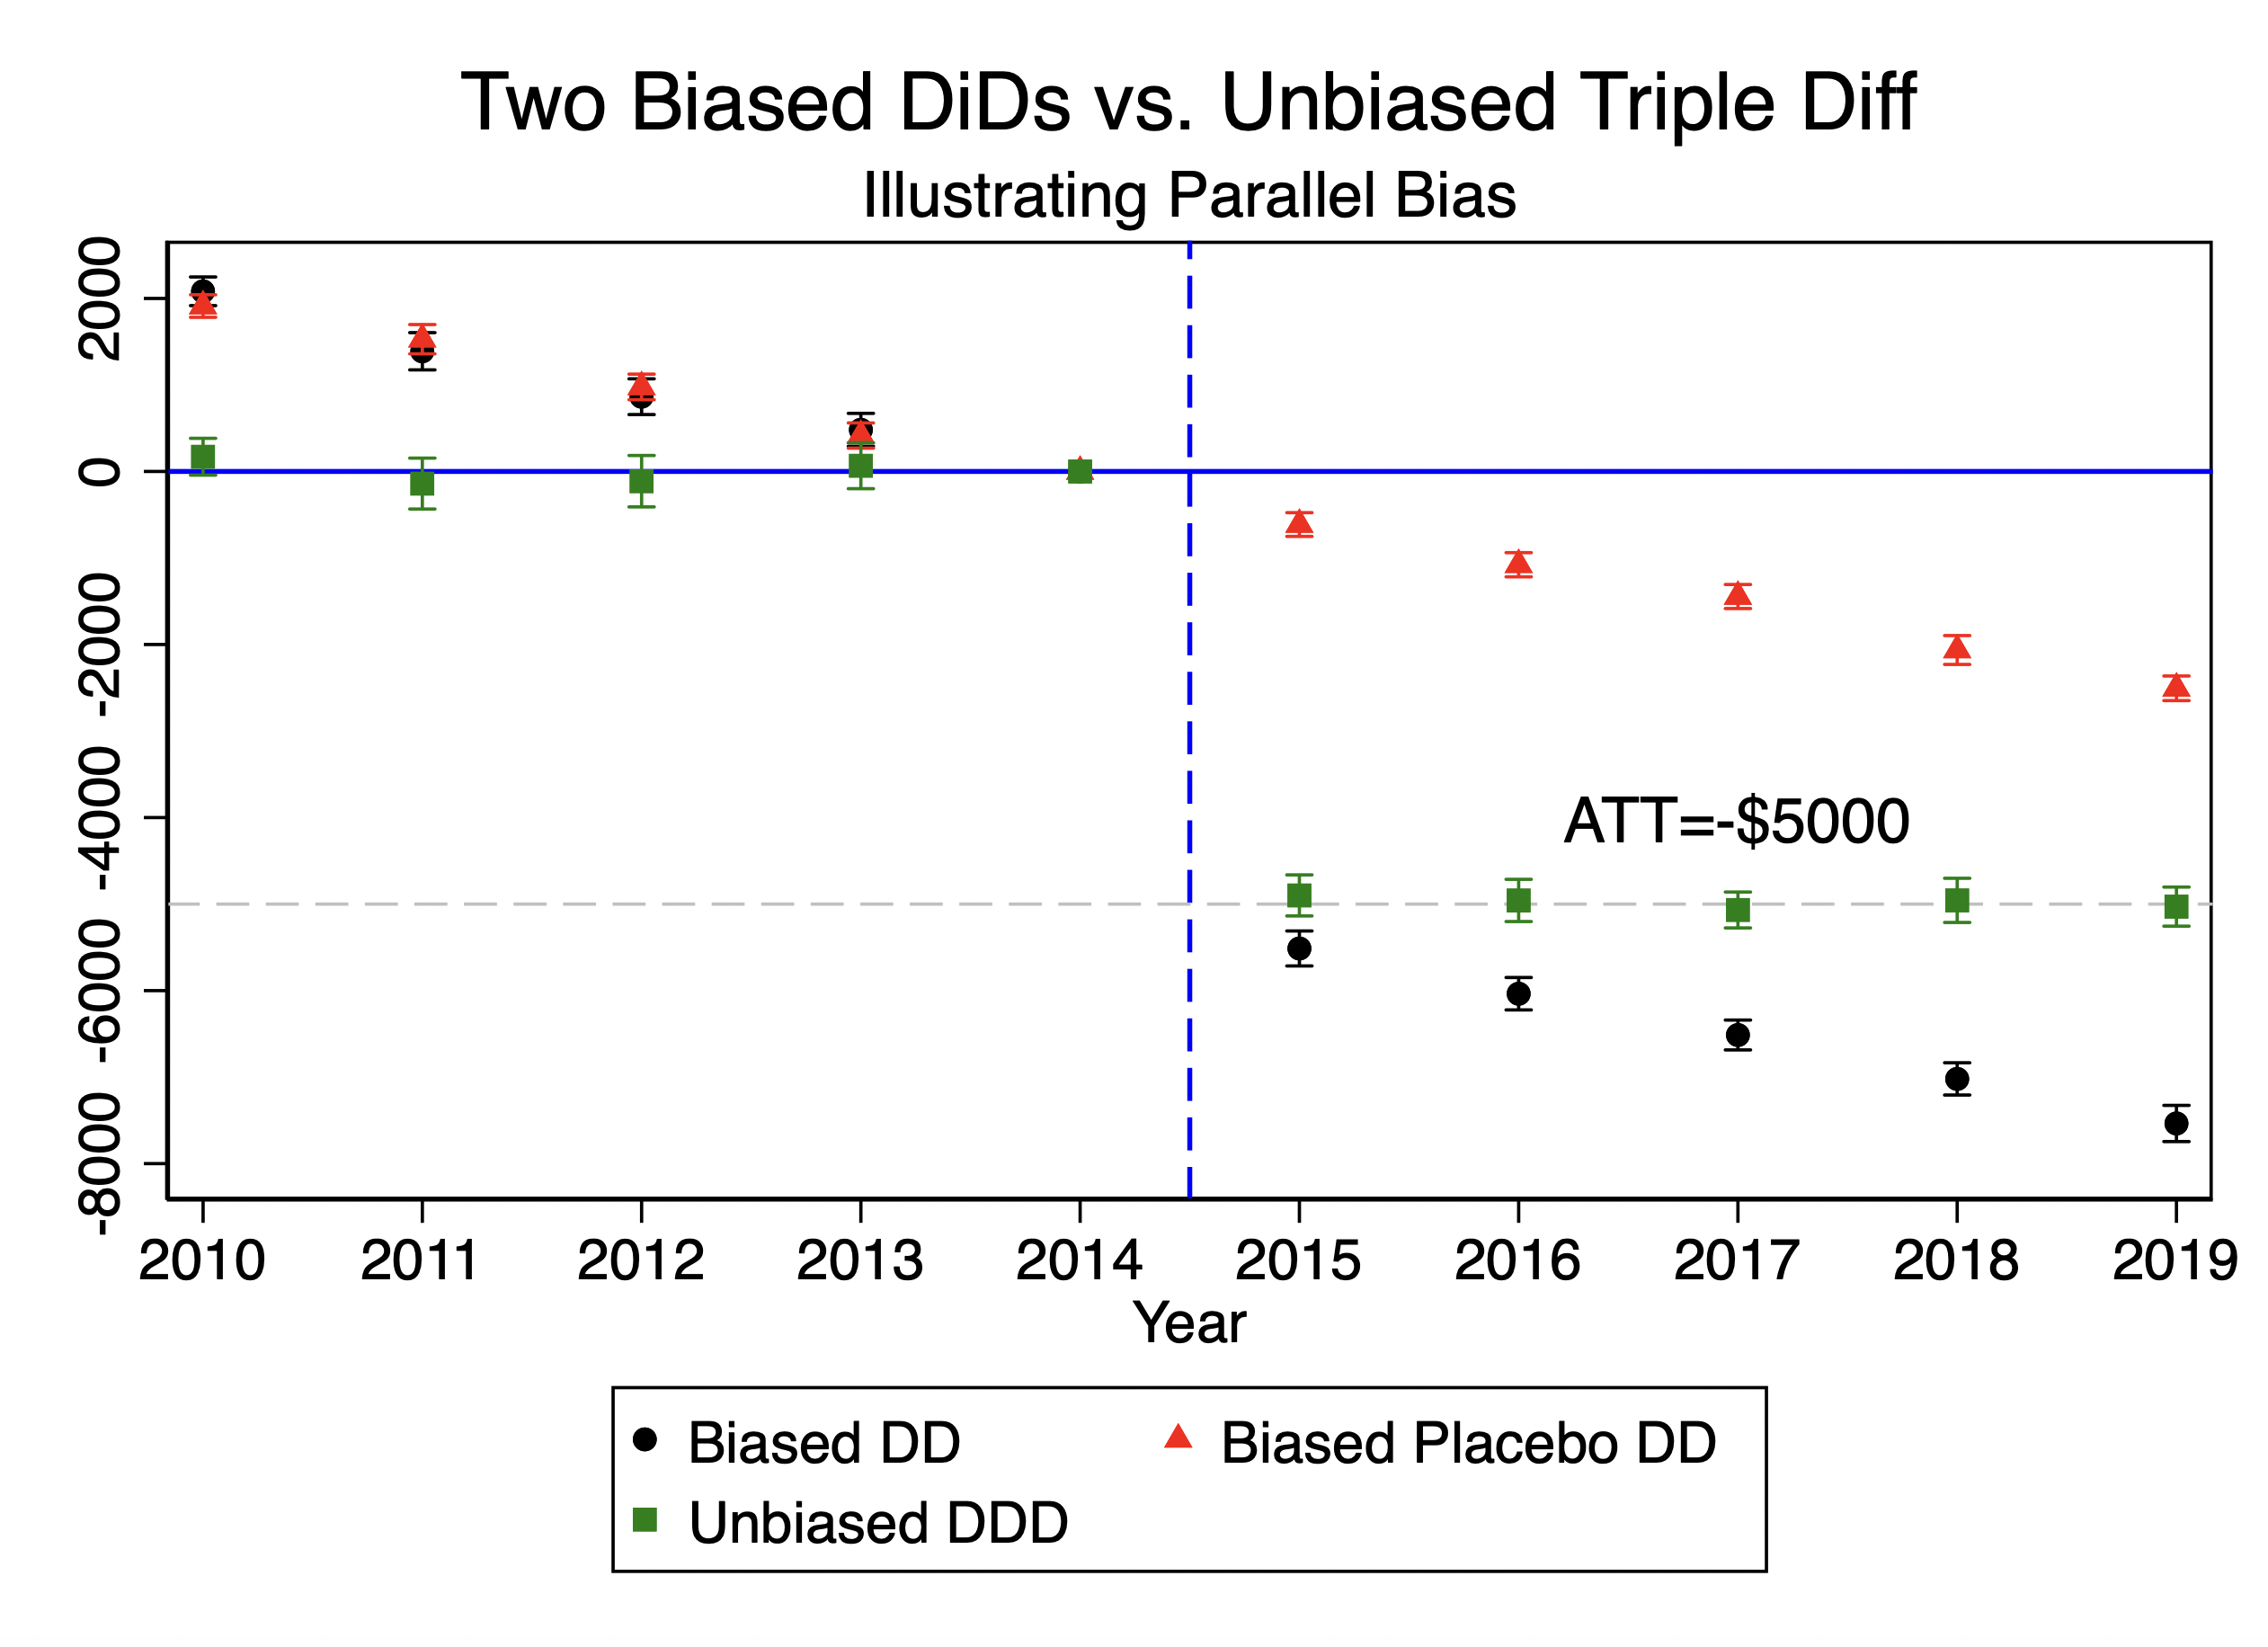
\includegraphics[scale=0.25]{./lecture_includes/ddd_simulation}
\end{figure}



\end{frame}  

\begin{frame}{Great new paper to learn more}

\begin{figure}

\includegraphics[scale=0.25]{./lecture_includes/olden_moen_2022_ddd.png}
\end{figure}

\end{frame}


\begin{frame}{Summarizing DDD}

\begin{itemize}
\item Used to be people thought DDD required two parallel trends assumptions but it does not -- it is a real design and requires one parallel trends assumption
\item Parallel trends assumption is ``parallel bias'' -- that the bias of the true DiD is the same as the bias of the placebo DiD
\item The ladder of evidence still holds -- you'll want to present the event study plot, and my code provides it for you, because you need to evaluate the parallel bias assumption
\item Given the lack of triple diff literacy, you may have to write this anticipating reader and maybe editor confusion and so "educate" as you go -- overlaying all three plots could be help

\end{itemize}

\end{frame}


\subsection{Falsifications}

\begin{frame}{Falsification with similar groups}

\begin{itemize}

	
	\item Recall that Miller, Johnson and Wherry (2021) found a very similar group to their near elderly population (i.e., the 65 and older)  as a falsification to provide evidence for parallel trends
	\item Evidence, again, is not proof -- could still be that the confounder is unique to the treatment group (i.e., the near elderly)
	\item Ideal falsification is a group that is ``almost'' the treatment group and use the same outcome and the same model
	\item Another example is Cunningham, DeAngelo and Tripp (2024) looked at the effect of Craigslist's erotic services on male homicides
\end{itemize}
\end{frame}

\begin{frame}{Falsifications on 65 year old and older}

	\begin{figure}
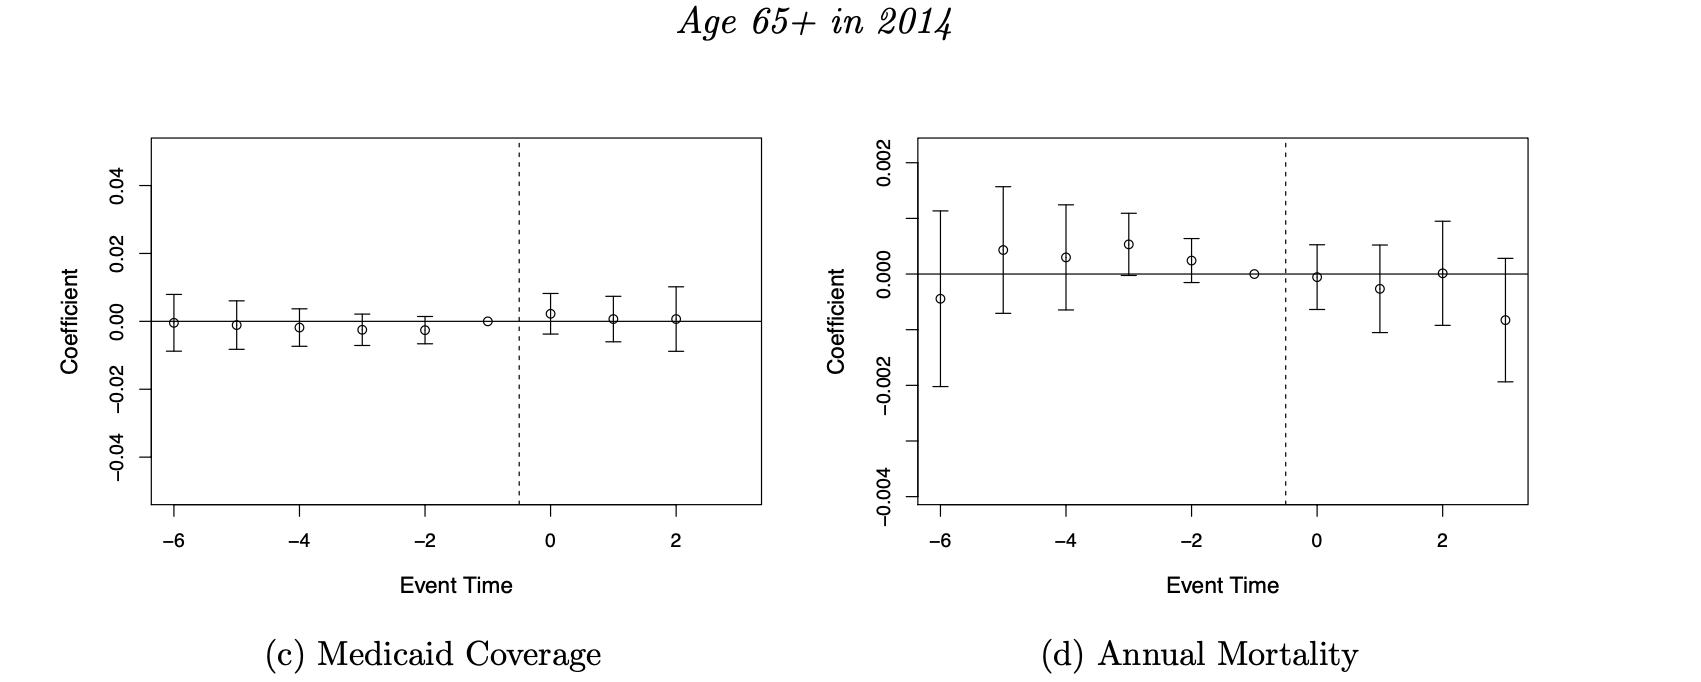
\includegraphics[scale=0.425]{./lecture_includes/placebo_medicaid}
	\end{figure}

\end{frame}


\begin{frame}{Falsifications with Different Outcomes}
\begin{itemize}
	\item Usually you have in mind a general confounder affecting many outcomes, not just your outcome.
	\item Falsifications are helped when there are specific confounders you have in mind that are consistent with your hypothesis but affect other things your hypothesis is unrelated to
	\item Cheng and Hoekstra (2013) examine the effect of castle doctrine gun laws on non-gun related offenses like grand theft auto and find no evidence of an effect 
	\item Cunningham, DeAngelo and Tripp (2024) looked at assaults as a falsification against our main result of female victimization
	\end{itemize}
\end{frame}



\begin{frame}{Example 1: Falsifications as a Critique of Rational Addiction}


Sometimes, an empirical literature may be criticized using nothing more than placebo analysis

\begin{quote}``A majority of [our] respondents believe the literature is a success story that demonstrates the power of economic reasoning.  At the same time, they also believe the empirical evidence is weak, and they disagree both on the type of evidence that would validate the theory and the policy implications. Taken together, this points to an interesting gap.  On the one hand, most of the respondents claim that the theory has valuable real world implications.  On the other hand, they do not believe the theory has received empirical support.''
\end{quote}

\end{frame}

\begin{frame}{Placebo as critique of empirical rational addiction}

\begin{itemize}
	\item Auld and Grootendorst (2004) estimated standard ``rational addiction'' models (Becker and Murphy 1988) on data with milk, eggs, oranges and apples.  
	\item They find these plausibly non-addictive goods are addictive, which casts doubt on the empirical rational addiction models.
\end{itemize}

\end{frame}

\begin{frame}{Example 2: Falsification as critique of peer effects}

\begin{itemize}
	\item Several studies found evidence for ``peer effects'' involving inter-peer transmission of smoking, alcohol use and happiness tendencies
	\item Christakis and Fowler (2007) found significant network effects on outcomes like obesity
	\item Cohen-Cole and Fletcher (2008) use similar models and data and find similar network ``effects'' for things that \emph{aren't} contagious like acne, height and headaches
	\item Homophily (sorting) is probably just as likely an explanation
\end{itemize}

\end{frame}

\begin{frame}{Concluding the basics}


\begin{itemize}

\item That concludes the core of diff-in-diff
\item A lot of what we just went through is pretty standard and common to any diff-in-diff, but some of it even other studies too
\item But what if actually doesn't hold and we can't fix it with triple differences or if the bounds are too large to be informative?  
\item Next we look at one very common example -- the use of covariates to fix parallel trends violations

\end{itemize}

\end{frame}


\end{document}


\subsection{Compositional Changes and Cross Sections}



\begin{frame}{Repeated cross-sections and compositional change}
	
	\begin{itemize}
	\item One of the risks of a repeated cross-section is that the composition of the sample may have changed between the pre and post period in ways that are correlated with treatment
	\item Hong (2013) uses repeated cross-sectional data from the Consumer Expenditure Survey (CEX) containing music expenditure and internet use for a random sample of households
	\item Study exploits the emergence of Napster (first file sharing software widely used by Internet users) in June 1999 as a natural experiment
	\item Study compares internet users and internet non-users before and after emergence of Napster
	\end{itemize}

\end{frame}

\begin{frame}{Introduction of Napster and spending on music}
	\begin{figure}
	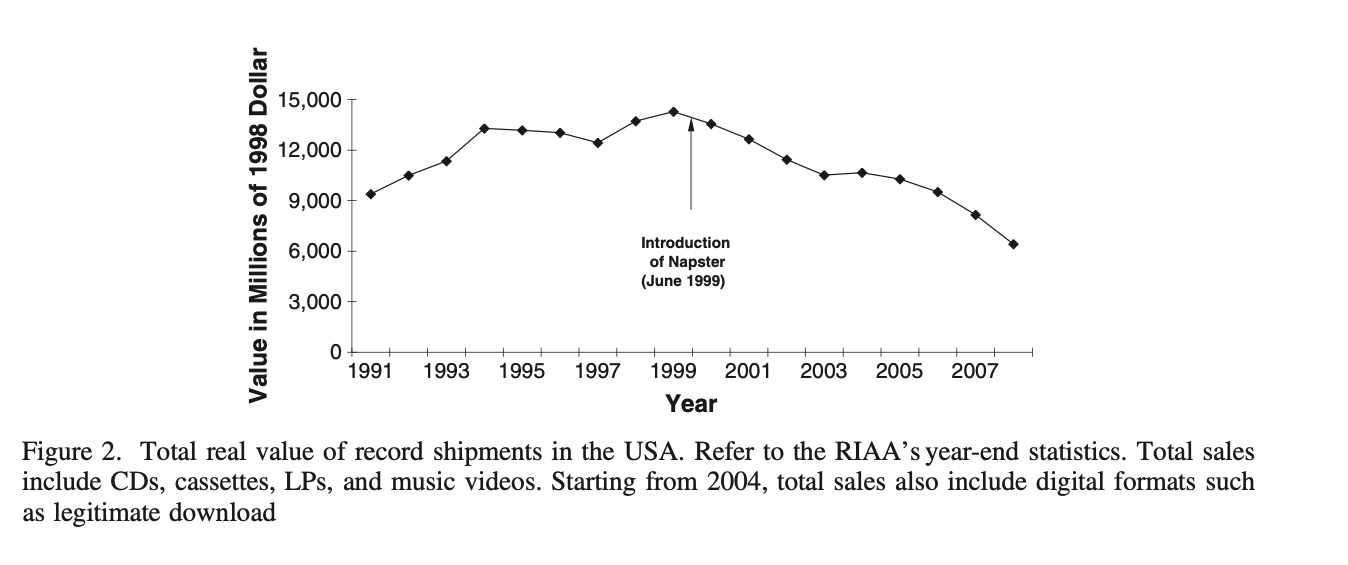
\includegraphics[scale=0.5]{./lecture_includes/hong_napster}
	\end{figure}
	
\end{frame}


\begin{frame}[plain]
	\begin{figure}
	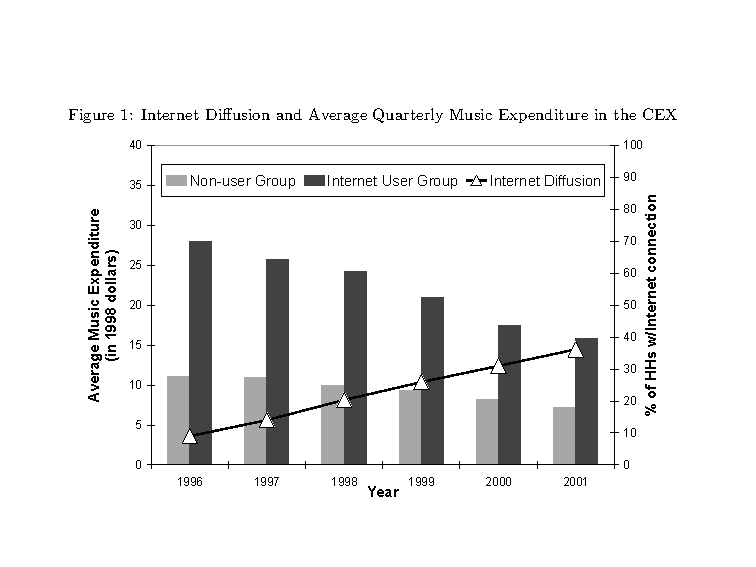
\includegraphics{./lecture_includes/Hong_1.pdf}
	\end{figure}
	
\end{frame}





\begin{frame}[shrink=20,plain]
	\begin{figure}
	\includegraphics{./lecture_includes/Hong_2.pdf}
	\end{figure}
	
	Diffusion of the Internet changes samples (e.g., younger music fans are early adopters)
	
\end{frame}

\begin{frame}{Repeated cross-sections}

\begin{itemize}
\item Surprisingly underappreciated problem with almost no literature around it
\item Replace the outcome with your time-varying covariates and estimate your DiD model
\item Use covariates highly predictive of the missing $E[Y^0|D=1]$ for this exercise
\item ``Difference-in-differences with Compositional Changes'' by Pedro Sant'Anna and Qi Xu is an update to Hong (2013)
\end{itemize}

\end{frame}

